% Arquivo editável que gera o pdf
% Copyright (C) 2018  Daniel Saad Nogueira Nunes (daniel.nunes@ifb.edu.br)

% This program is free software: you can redistribute it and/or modify
% it under the terms of the GNU General Public License as published by
% the Free Software Foundation, either version 3 of the License, or
% (at your option) any later version.

% This program is distributed in the hope that it will be useful,
% but WITHOUT ANY WARRANTY; without even the implied warranty of
% MERCHANTABILITY or FITNESS FOR A PARTICULAR PURPOSE.  See the
% GNU General Public License for more details.

% You should have received a copy of the GNU General Public License
% along with this program.  If not, see <http://www.gnu.org/licenses/>.


\documentclass[pt]{ifbclass/apresentacao-ifb}
\usepackage{natbib} 
\usepackage[brazil]{babel}
\usepackage{amsmath}
\usepackage{amssymb}% http://ctan.org/pkg/amssymb
\usepackage{pifont}% http://ctan.org/pkg/pifont
\newcommand{\cmark}{\ding{51}}%
\newcommand{\xmark}{\ding{55}}%

\usepackage{multirow}

% Insira os dados aqui
\author{Danyelle da Silva Oliveira Angelo}
%\orientador{Daniel Saad Nogueira Nunes}
%\orientador{Prof.\ Me.\ Daniel Saad Nogueira Nunes}
\title{Uma proposta de Range min-Max tree k-ária para consultas sobre árvores sucintas}
%\subtitle{Subtítulo}
\institute{Instituto Federal de Brasília, Câmpus Taguatinga}
\date{14 de setembro de 2021}



\AtBeginSection[]
{
\begin{frame}<beamer>
	\frametitle{Sumário}
	\tableofcontents[currentsection,sectionstyle=show/hide,subsectionstyle=show/shaded/hide]
\end{frame}
}

\AtBeginSubsection[]
{
	\begin{frame}<beamer>
	\frametitle{Sumário}
	\tableofcontents[sectionstyle=show/hide,currentsubsection]
\end{frame}
}

\begin{document}
\maketitle

\begin{frame}{}
	\frametitle{Sumário}
	\tableofcontents[sectionstyle=show/show]
\end{frame}


\chapter{Introdução}
\label{chp:introduction}

A cada ano novas aplicações e dispositivos com formatos e recursos diversos são lançados no mercado, o crescimento de aplicações como as de transporte, dos serviços de streamings, a popularização de  dispostivos IoT, o crescimento dos datacenters e do serviço em nuvem vêm contribuindo fortemente para o aumento na produção de dados \citep{relatorio-idc}.

Especializada em computação em nuvem, a \citeauthor{domo-study} realiza anualmente uma análise da quantidade de informação produzida na internet  a cada \textit{minuto}. Abaixo vemos algumas das estatísticas relativas à esse estudo \citep{domo-study}:

\begin{itemize}
    \item 41.666.667 mensagens são enviadas através do aplicativo de mensagens WhatsApp;
    \item 479.452 pessoas interagem com conteúdos da plataforma Reddit;
    \item 208.333 pessoas participam de conferências no serviço de chamada Zoom, ao passo que o Microsoft Teams conecta cerca de 52.083 usuários por minuto;
    \item 147.000 uploads de fotos são feitos no Facebook e 150.000 mensagens são enviadas na mesma plataforma;
    \item 28 faixas de música são incluídas no serviço de streaming Spotify;
    \item 500 horas de vídeos são enviadas ao youtube.
\end{itemize}

Prevê-se que, essa quantidade de dados irá crescer nos próximos anos. De acordo com o relatório anual da \citet{relatorio-cisco}, em 2018 o número de usuários conectados à internet era de 3,9 bilhões, até 2023 mais de 70\% da população terá acesso à internet, atingido a marca de 5,3 bilhões de usuários conectados. A International Data Corporation (IDC) prevê que em 2025, 75\% (6 bilhões) da população mundial interaja com aplicações diversas todos os dias, fazendo com que a quantidade de dados produzidos cresça de 33 Zetabytes (ZBs) em 2018, para 175 ZBs em 2025 \citep{relatorio-idc}.

Esse crescimento na produção de dados tem relação direta com o surgimento de novos dispositivos. O grande problema é que existe uma lacuna de
desempenho entre CPU e memória. Essa lacuna se deve principalmente ao fato de que os fabricantes de processadores estão focados em obter uma lógica rápida,  que acelera a comunicação, ao passo que os fabricantes de memória objetivam uma capacidade de armazenamento de dados maior \citep{paper-processor-memory-bottleneck}. Essa disparidade é um grande desafio para projetitas e desenvolvedores, pois como afirmam \citet{paper-processor-memory-bottleneck},  esta faz com que seja criado um atraso na comunicação entre CPU e memória (conhecido gargalo de Von-Neumann), sobretudo quando se trabalha com um grande conjunto de dados. Diversas soluções foram e estão sendo desenvolvidas para contornar o problema dessa lacuna, entre elas o uso de computação paralela em nível de instrução, hierarquia de memória multinível, \textit{smarter memories}, técnicas específicas de tolerância à latência, e compressão de dados \citep{paper-Processor-Memory-bottleneck-Problems-Solutions, paper-processor-memory-bottleneck}.

Como mostra \cite{book-compact-data-structures}, estruturas de dados sucintas são uma forma de compressão de dados. Elas representam a informação de maneira eficiente, usando um espaço próximo ao limite inferior estabelecido pela Teoria da Informação, possibilitando ainda operações sobre seus objetos de modo que não seja necessário que estes sejam descompactados, o que a torna mais eficiente do que os algoritimos de compactação  clássicos que precisam de armazenamento e tempo extra para descompactar os objetos sobre os quais operam.  Esses fatores fazem com que as estruturas de dados sucintas sejam amplamente usadas em sistemas como os de mecanismo de busca,  ou sistemas que trabalham com dados geográficos. Estruturas de dados sucintas também são essenciais para lidar  com dispositivos em que a quantidade de memória é limitada, como  dispositivos IoTs e embarcados \citep{book-compact-data-structures}. %Por fim, mesmo que seja necessário reter parte do conjunto de dados em um nível mais baixo da hierarquia de memória, onde o tempo para obter uma informação é maior, o uso de estruturas de dados sucintas ainda possibilitará aplicações eficientes, haja vista que o seu uso minimizará o número de acessos a  memórias mais lentas.

Com os dados residindo em memória principal, temos um novo gargalo, dessa vez entre memória cache e memória principal. Nesse sentido e tendo em vista a lacuna de desempenho crescente entre processador e memória RAM, faz-se necessário buscarmos formas de melhor utilizarmos a cache.  \citet{paper-making-btree-cache} implementaram em um de seus trabalhos, diferentes versões de uma estrutura denominada \textit{Cache-Sensitive Search Trees (CSS-Tree)}, a \textit{Cache-Sensitive B$^+$-Tree (CSB$^+$-Tree)}, que tem como objetivo melhorar o desempenho de operações de atualização existentes na \text{CSS-tree}, através da maximização da quantidade de dados em cada nó. Durante os experimentos foi constatado que a estrutura original apresentava melhor desempenho nas operações de pesquisa devido ao seu alto fator de ramificação, se comparado ao da \textit{CSB$^+$-tree}. Foi observado também que entre as diferentes versões da \text{CSB$^+$-tree} implementadas, os autores obtiveram melhor desempenho, tanto em operações de atualização, como de pesquisa, nas versões que tinham fator de ramificação mais alto.

Nesse trabalho, nos concentraremos no estudo de árvores, uma das estruturas mais populares no campo da Ciência da Computação. De acordo com \citet{paper-succint-trees-in-practice}, no caso das árvores sucintas, as diferentes versões existentes na literatura podem diferir em sua funcionalidade, variando daquelas que suportam navegação de um nó filho para um nó pai ou aquelas que suportam operações como obter o ancestral comum mais baixo de dois nós, até aquelas que suportam um conjunto completo de operações, podendo variar em relação ao espaço ocupado, indo  de $O(n/(\log \log n)^2)$ à $O(n/ polylog(n))$ bits.

A nossa contribuição consiste na proposta de uma versão alternativa, de uma estrutura de dados sucinta já existente: a range min-Max tree (rmM-tree), de \cite{paper-fully-functinal-succint-trees}. Essa estrutura fornece suporte à diversas operações sobre árvores compactas. Em sua versão estática, ela pode ser construída usando apenas $n + O(\frac{n}{b} \log n)$ bits de espaço, sendo capaz de realizar operações em tempo $O(\log n)$\citep{paper-fully-functinal-succint-trees}. Essa estrutura é construída no formato de uma árvore binária completa, e portanto, possuí um baixo fator de ramificação. Assim, com base no exposto por \citet{paper-making-btree-cache}, propomos então uma versão da rmM-tre binária, no formato de árvore k-ária, afim de maximizar o fator de ramificação da range min-Max tree. Nossa estrutura se baseia também em um número maior de entradas por nó, visando aumentar o volume de dados enviados a cache em cada transferência, aproveitando do a localidade espacial\footnote{"itens cujos endereços estão próximos um do outro costumam ser referenciados em curto espaço de tempo" \citep{book-computer-architecutre}}, o que pode melhorar significativamente o desempenho de sistemas de buscas que lidam com grandes quantidade de dados.



% \section{Metodologia}
% Esse estudo será feito com base na revisão bibliográfica da estrutura proposta por \citet{paper-fully-functinal-succint-trees}, visando melhor entendimento das operações de navegação e consulta sobre árvores. Implementaremos a versão original da rmM-tree, buscando abranger todas as operações suportadas na literatura, além da versão original será implementada a versão alternativa da rmM-tree, no formato de árvore k-ária, com até k entradas por nó. Para realizar a validação das nossas implementações, usaremos a biblioteca \textit{Succint Data Structure Library (SDSL)}, uma biblioteca construída em C++, com código aberto e de alta qualidade, que reúne os destaques de $40$ publicações de pesquisa \citep{sdsl-article}. Auxiliará na validação das respostas das estruturas implementadas o framework Google Tests. Já o desempenho das estruturas será analisado mediante o uso do framework Google Benchmark.



\section{Estrutura do documento}
De modo a atingir os objetivos citados, o Capítulo~\ref{ch:fundamentacao} traz um estudo sobre hierarquia de memória, estrutura de dados sucintas e as características e operações suportadas pela range min-Max tree, ao final deste capítulo trazemos uma discussão acerca do aproveitamento efetivo da cache. O Capítulo~\ref{chp:desenvolvimento} apresenta a nossa versão da rmM-tree k-ária, expondo suas principais características e diferenças em relação à estrutura clássica. O Capítulo~\ref{chp:resultados}, discorre a respeito dos testes experimentais, metodologia usada para os mesmos e resultados alcançados. Por fim o Capítulo~\ref{chp:conclusao} expõe as nossas conclusões em relação 
aos objetivos e resultados alcançados, bem como as nossas perspectivas em relação aos trabalhos futuros.
%contextualizar a representação sucinta de dados, falar de maneira menos técnica questões de memória. Estruturas sucintas de modo geral, uma delas são as árvores sucintas, trazer exemplos de aplicações. Para que servem as árvores, que tipo de aplicação são usadas.
%deixsr claro a proposta
%manter objetivos

%\figref{fig:research-methodology-thesis} shows
%the multimethod research design applied in this thesis.
%\begin{figure}[h]
%\centering
%  \caption[Research methodology.]{The research methodology applied for this
%  thesis.}
%  \includegraphics[width=\columnwidth]{images/research-methodology-thesis.pdf}
%  \footnotesize{Source: Made by the author.}
%  \label{fig:research-methodology-thesis}
%\end{figure}


\section{Fundamentação teórica}

\begin{frame}{Estrutura de dados sucintas}
Estrutura de dados sucintas são uma forma de compressão de dados, e de acordo com \cite{book-compact-data-structures}, estas propiciam:
\begin{itemize}
    \item Representação dos objetos obedecendo o limite da entropia da informação;
    \item Operações eficientes em questões de tempo e espaço;
    \item Manipulação de dados em dispositivos com memória limitada;
\end{itemize}
\end{frame}

\begin{frame}{Vetores de bits - access}
    Sequência de $n$ elementos sobre o alfabeto $\Sigma = \{0,1\}$, no qual podem ser realizadas as seguintes operações \citep{book-compact-data-structures}:
        \vspace{0.5cm}
        \begin{itemize}
            \item $access(BV,i)$: retorna o i-ésimo bit do vetor BV, com $0 \leq i < n$;
            \vspace{0.5cm}
            
            Exemplo: $access(BV,10)$
            
            \begin{figure}[h!]
                \centering
                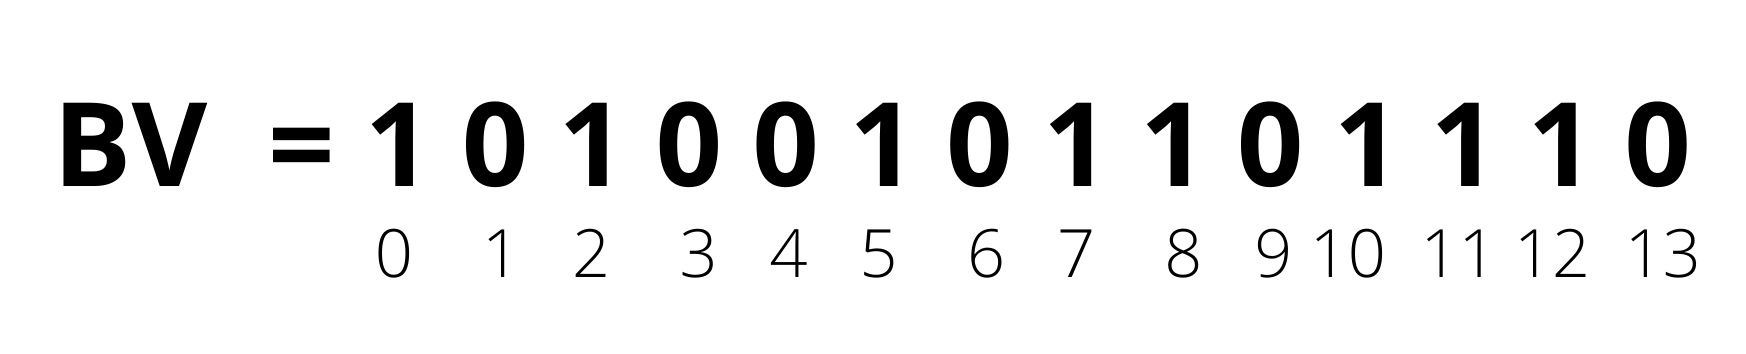
\includegraphics[scale=0.5]{images/bitvector.png}
            \end{figure} 
        \end{itemize}
    \end{frame}
    
    \begin{frame}{Vetores de bits - access}
        Exemplo: $access(BV,10)=1$
        \begin{figure}[h!]
            \centering
            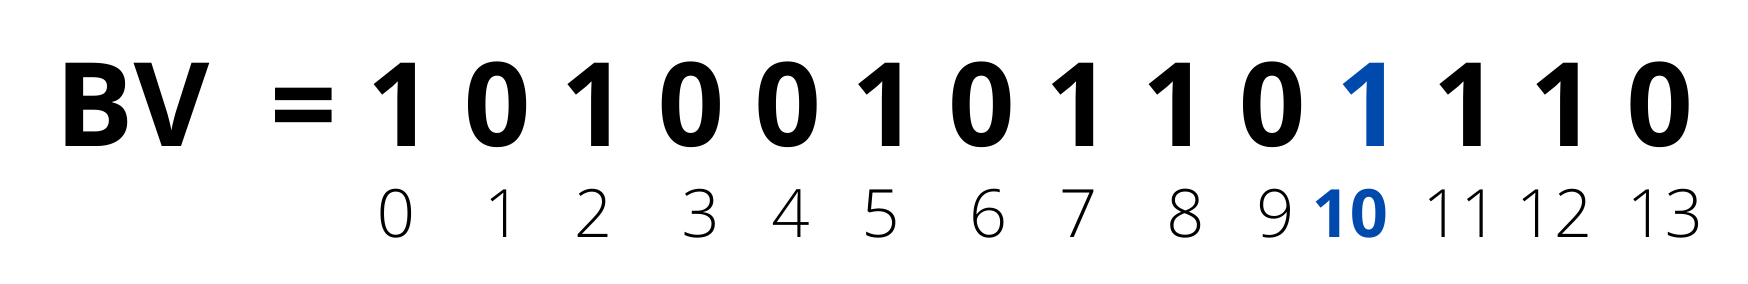
\includegraphics[scale=0.7]{images/access-res.png}
        \end{figure} 
    \end{frame}
    
    
    \begin{frame}{Vetores de bits - rank}
    Sequência de $n$ elementos sobre o alfabeto $\Sigma = \{0,1\}$, no qual podem ser realizadas as seguintes operações \citep{book-compact-data-structures}:
        \vspace{0.5cm}
        \begin{itemize} 
            \item $rank_v(BV,i)$: seja $v \in \{0,1\}$, e $0 \leq i < n$, retorna o número de ocorrências de $v$ no intervalo $BV[0,i]$.
            \vspace{0.5cm}
            
            Exemplo: $rank_0(BV,8)$
            
            \begin{figure}[h!]
                \centering
                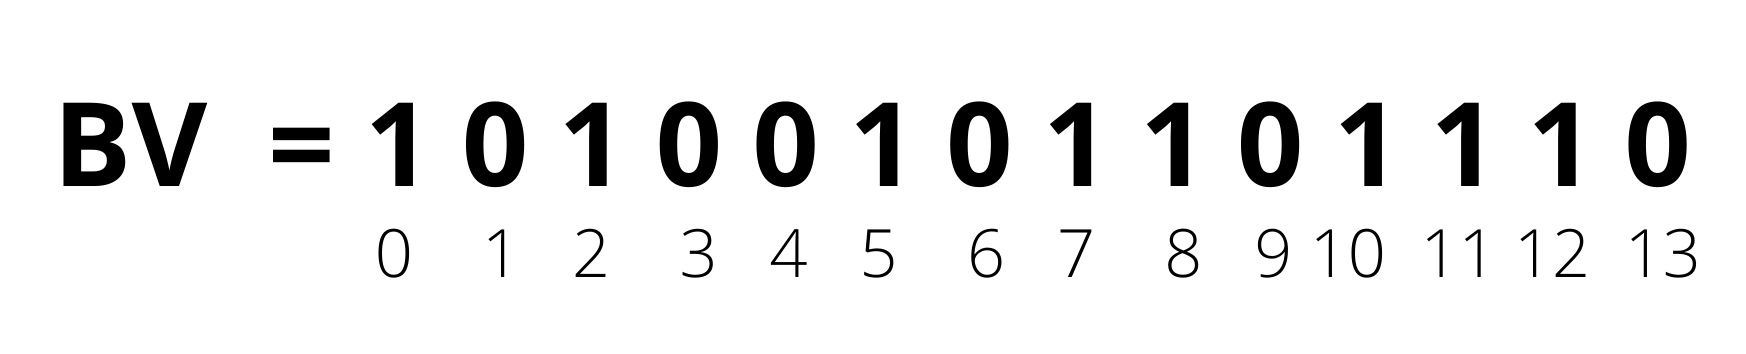
\includegraphics[scale=0.5]{images/bitvector.png}
            \end{figure} 
        \end{itemize}
    \end{frame}
    
    \begin{frame}{Vetores de bits - rank}
        Exemplo: $rank_0(BV,8)=4$
        \begin{figure}[h!]
            \centering
            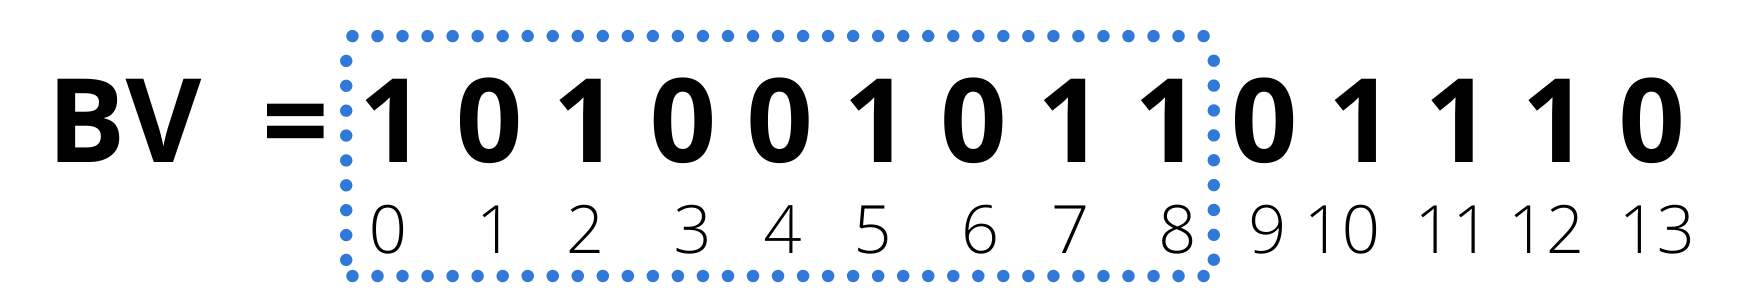
\includegraphics[scale=0.7]{images/rank-res.png}
        \end{figure} 
    \end{frame}
    
    \begin{frame}{Vetores de bits - select}
    Sequência de $n$ elementos sobre o alfabeto $\Sigma = \{0,1\}$, no qual podem ser realizadas as seguintes operações \citep{book-compact-data-structures}:
        \vspace{0.5cm}
        \begin{itemize} 
              \item $select_v(BV,i)$: dado $v \in \{0,1\}$ e $i \geq 0$, retorna a posição do i-ésimo bit $v$ em $BV[0,n-1]$.
              \vspace{0.5cm}
            
                Exemplo: $select_1(BV,7)$
            
                \begin{figure}[h!]
                    \centering
                    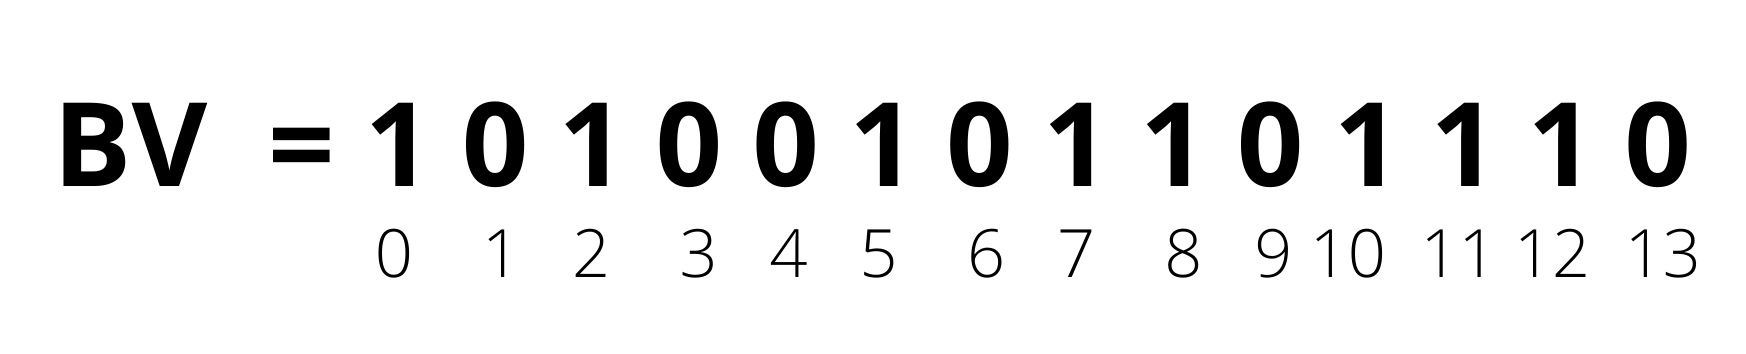
\includegraphics[scale=0.5]{images/bitvector.png}
                \end{figure} 
        \end{itemize}
    \end{frame}
    
    \begin{frame}{Vetores de bits - select}
        Exemplo: $select_1(BV,7)=12$
        \begin{figure}[h!]
            \centering
            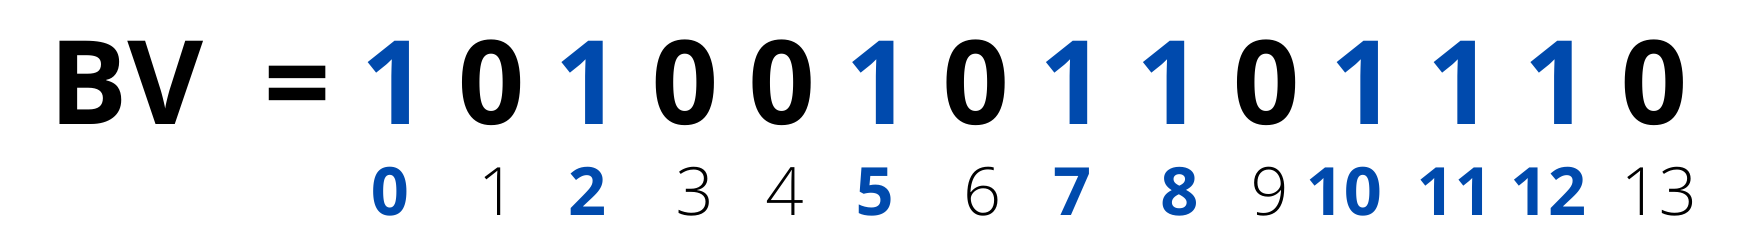
\includegraphics[scale=0.7]{images/select-res.png}
        \end{figure} 
    \end{frame}

\begin{frame}{Representações sucintas de árvores}
\begin{itemize}
    \item Parênteses balanceados (BP);
    \item Depth-First Unary Degree Sequence (DFUDS);
    \item Level-order Unary Degree Sequence (LOUDS);
\end{itemize}    
\end{frame}

\begin{frame}{Representações sucintas de árvores}
    \textbf{Representação de árvores sucintas via Parênteses Balanceados}
        \begin{figure}[h!]
            \centering
            
            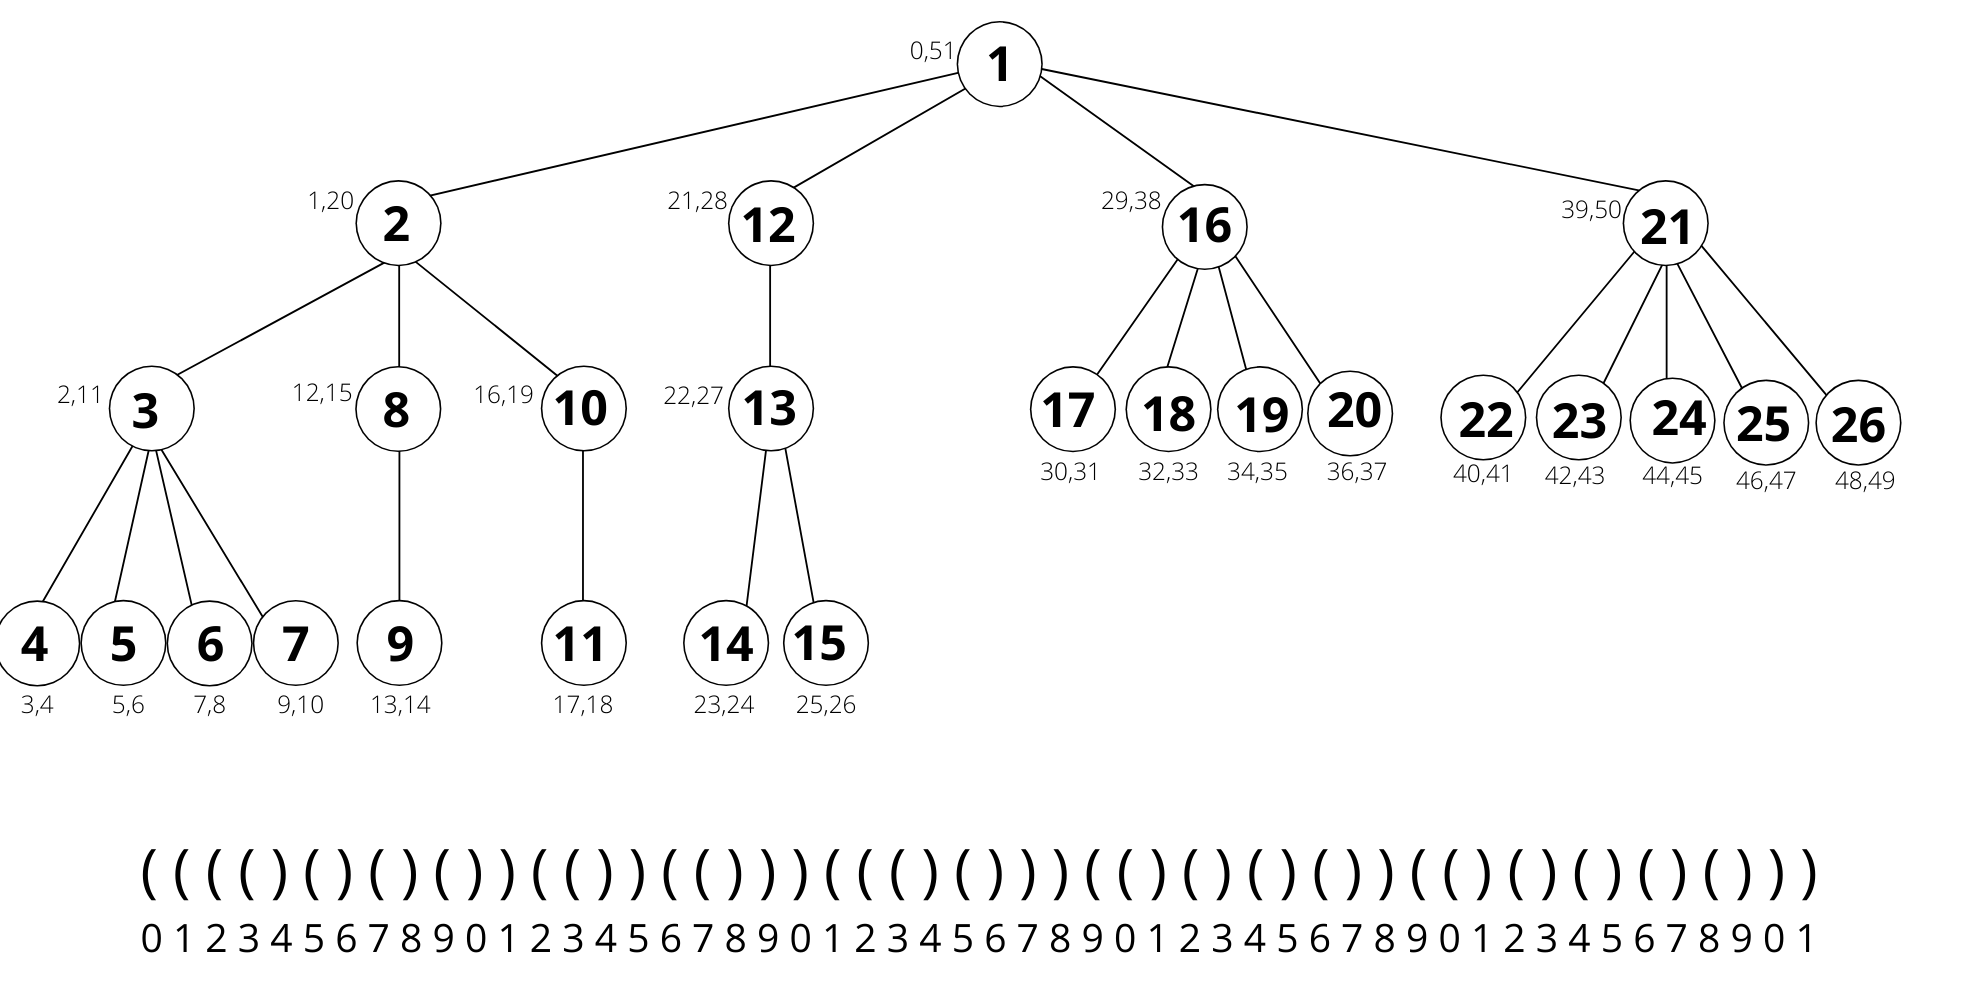
\includegraphics[scale=0.37]{images/arvore_geral.png}
        \end{figure} 
\end{frame}

\begin{frame}{Representações sucintas de árvores}
    \textbf{Representação de árvores sucintas via parênteses balanceados}
        \begin{itemize}
            \item Sequência de $2n$ parênteses balanceados;
            \item Complexidade de espaço $2n + o(n)$ bits;
            \item Através de estruturas auxiliares suporta:
            \begin{itemize}
                \item findclose(B,i);
                \item findopen(B,i);
                \item excess(B,i);
            \end{itemize}
        \end{itemize}
    \end{frame}
    
    \begin{frame}{Representações sucintas de árvores}
    Exemplo: \textit{excess(B,6) = -1}
        \begin{figure}[h!]
            \centering
            
            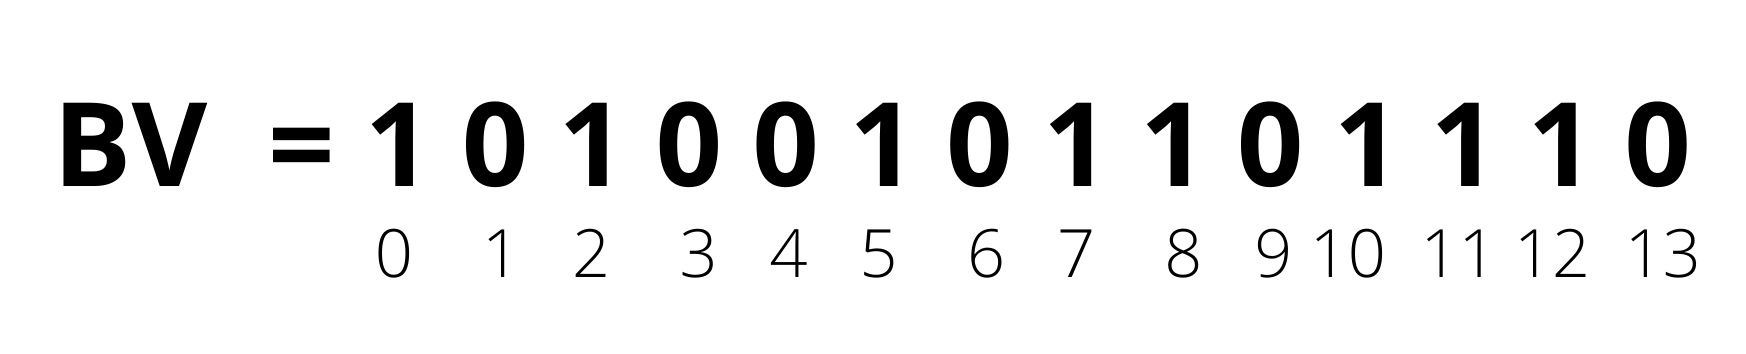
\includegraphics[scale=0.5]{images/bitvector.png}
        \end{figure} 
\end{frame}
\begin{frame}{Representações sucintas de árvores}
    \textbf{Representação de árvores sucintas via DFUDS}
        \begin{figure}[h!]
            \centering
            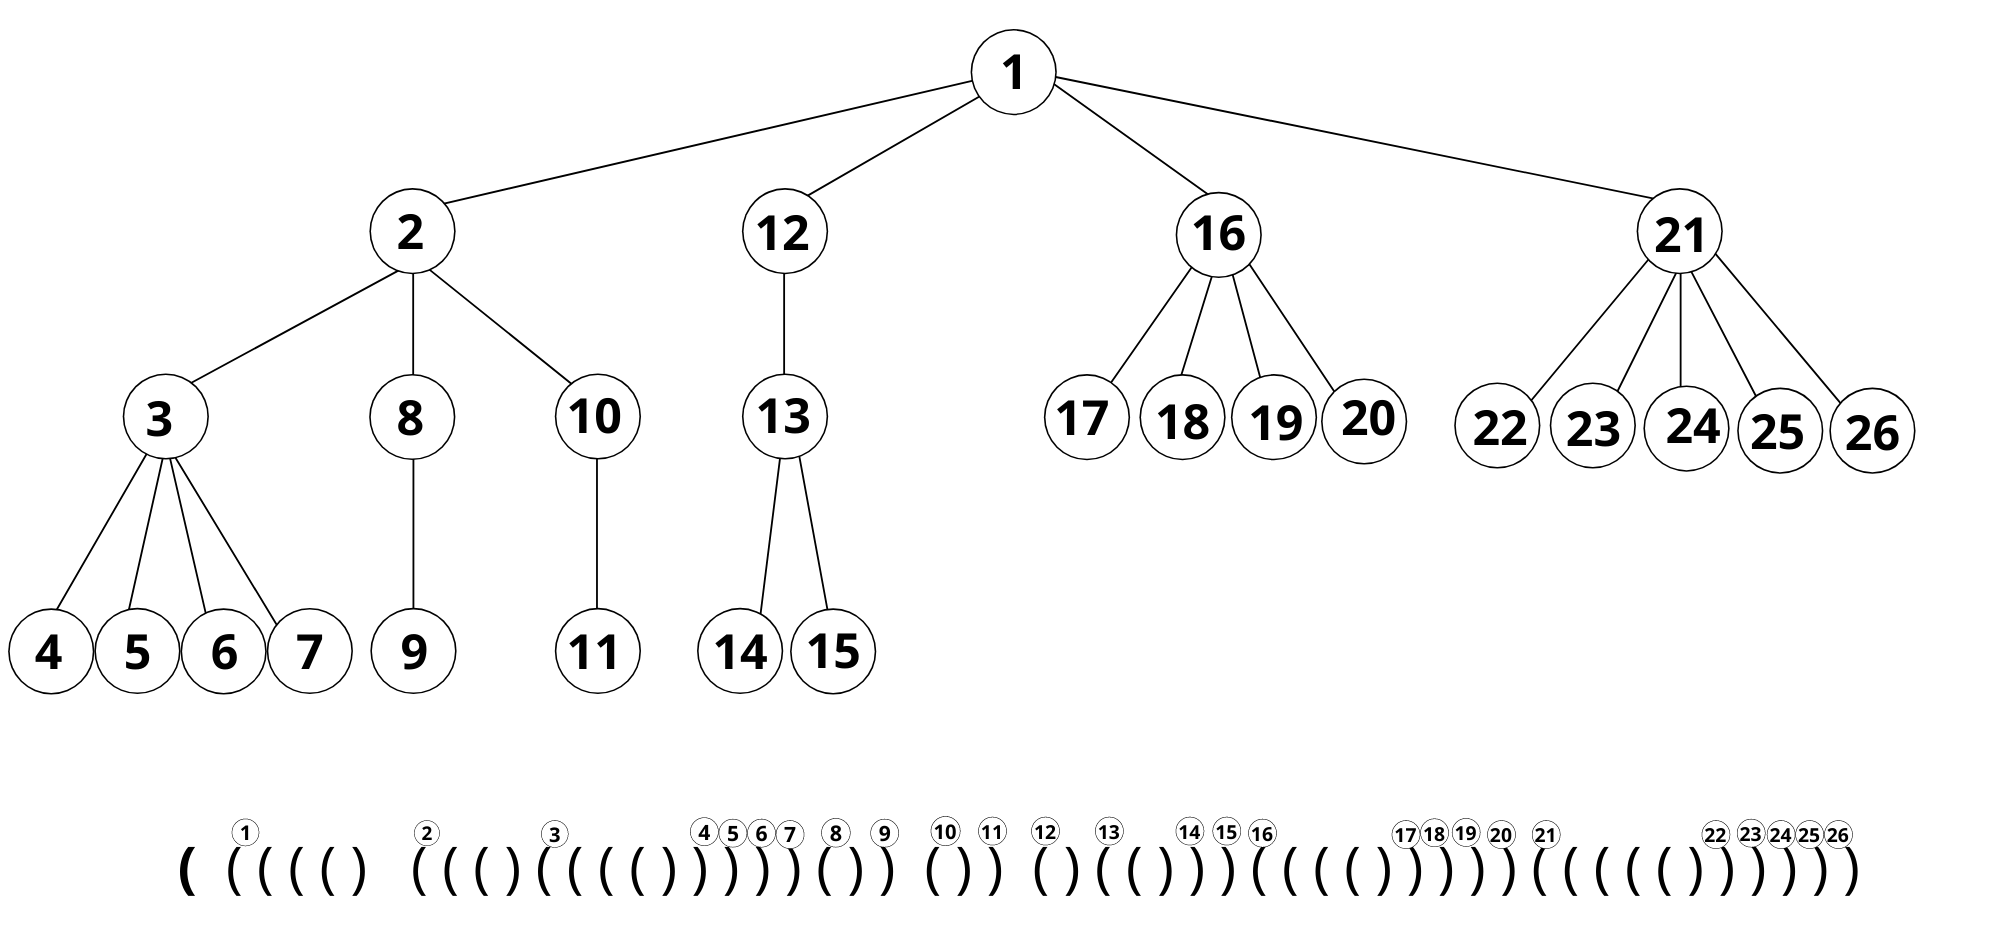
\includegraphics[scale=0.37]{images/dfuds.png}
        \end{figure} 
\end{frame}
\begin{frame}{Representações sucintas de árvores}
    \textbf{Representação de árvores sucintas via LOUDS}
        \begin{figure}[h!]
            \centering
            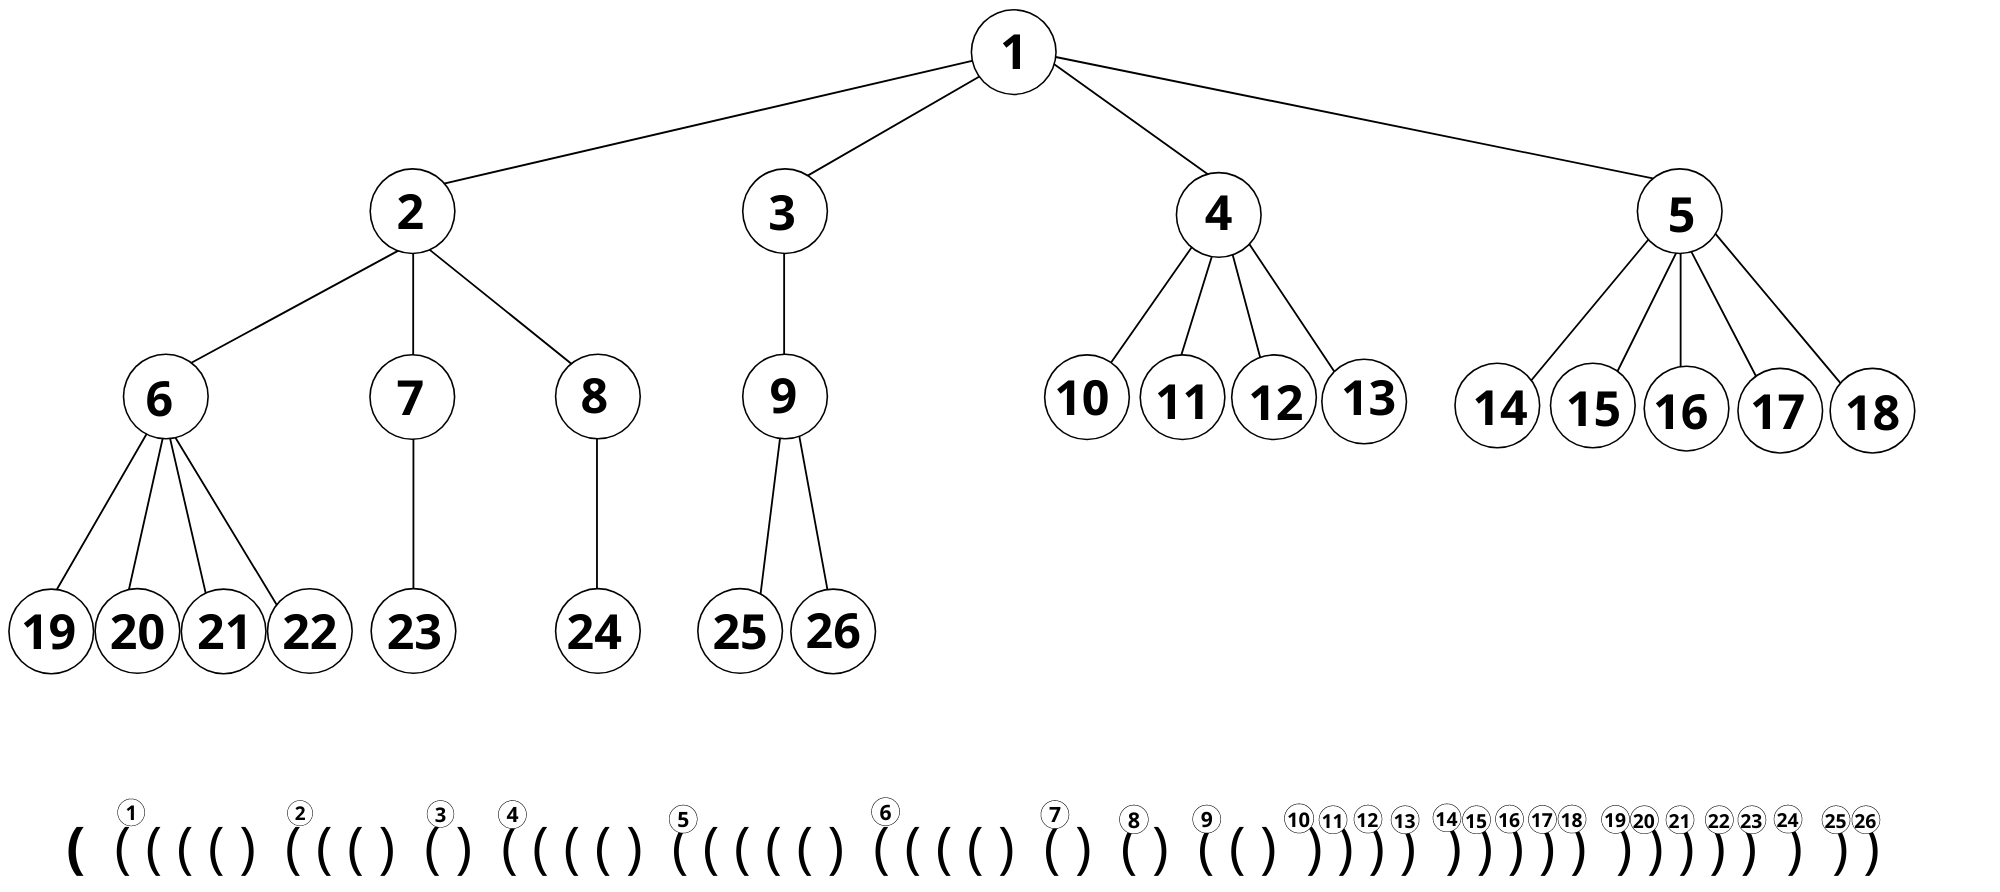
\includegraphics[scale=0.37]{images/louds.png}
        \end{figure} 
\end{frame}



\begin{frame}{range min-Max tree (rmM-tree)}
    \begin{itemize}
        \item Construção bottom-up;
        \item Árvore binária completa, baseada em intervalos de tamanho $b$;
        \item Cada nó cobre valores de excessos dentro de um intervalo;
        \item Complexidade de espaço igual à $n + O(\frac{n}{b} \log n)$ bits;
        \item Operações realizadas em tempo $O(\log n)$.
    \end{itemize}
\end{frame}

\begin{frame}{range min-Max tree binária}
    \begin{figure}[h!]
        \centering
        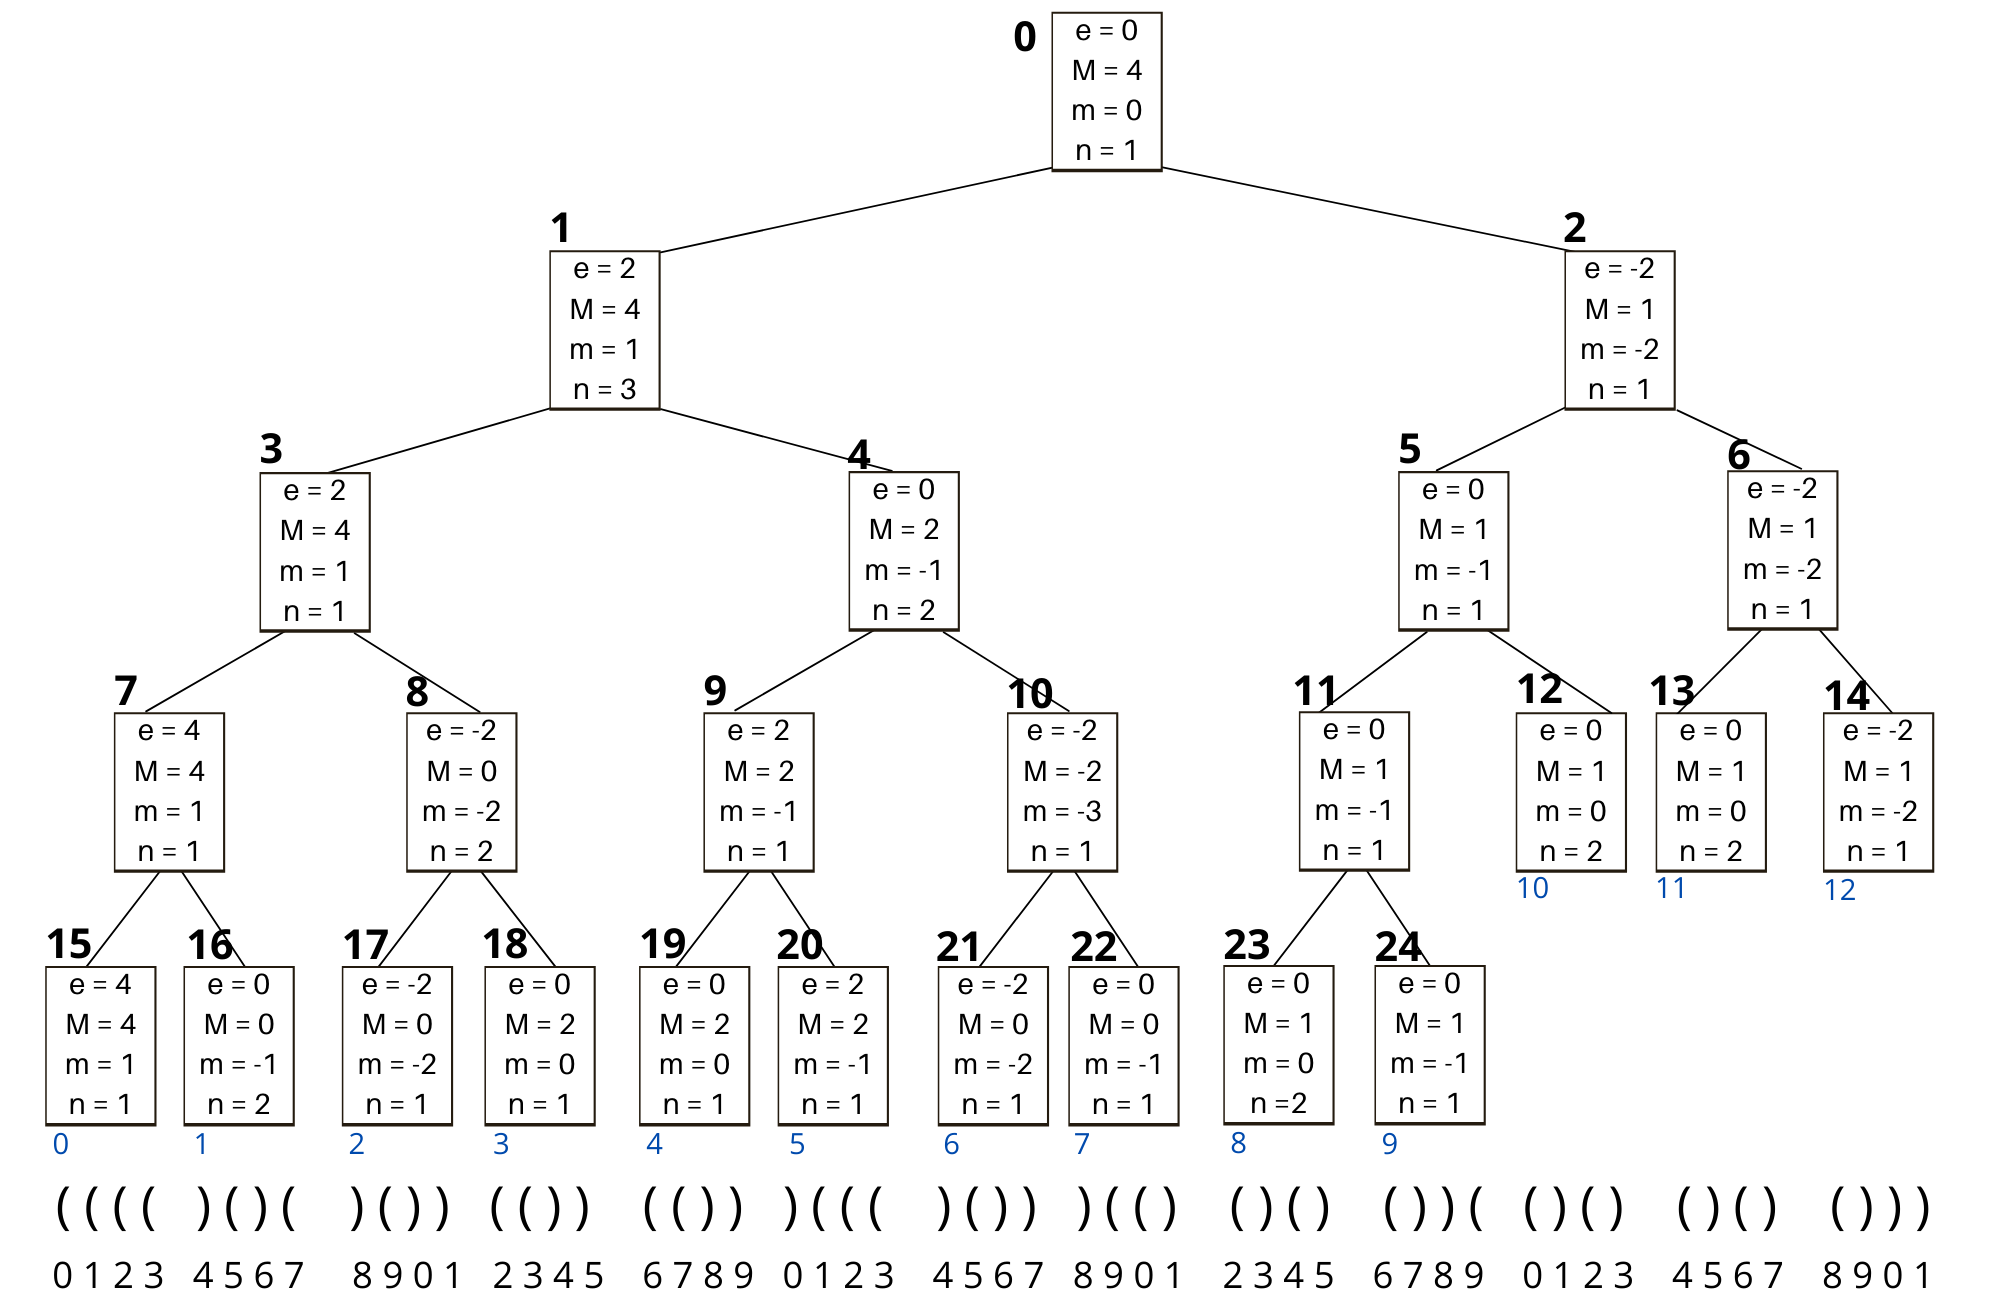
\includegraphics[scale=0.3]{images/rmm-tree-bin.png}\\
        \caption{rmM-tree binária com blocos de tamanho 4}
    \end{figure} 
\end{frame}

\begin{frame}{rmM-tree: Registros}

    \textbf{Valores de excesso}
        Dado um nó $v$ que cobre um intervalo $BP[s,e]$, então:
        \begin{itemize}
            \item $R[v].e$: excesso total no intervalo\\
            $R[v].e = excess(e)-excess(s-1)$.
            \item $R[v].M$: excesso máximo no intervalo\\
            $R[v].M = \max\{excess(i) - excess(s - 1) | s \leq i \leq e\}$.
            \item $R[v].m$: excesso mínimo no intervalo\\
            $R[v].m = \min\{excess(i) - excess(s - 1) | s \leq i \leq e\}$.
            \item $R[v].n$: número de vezes que o excesso mínimo ocorre no intervalo\\
            $R[v].n = |\{BP[i]=R[v].m | s \leq i \leq e\}|$.
        \end{itemize}
\end{frame}

\begin{frame}{rmM-tree: Registros}
    \textbf{Nós internos e raíz}
    \begin{figure}[h]
        \begin{minipage}[c]{0.35\linewidth}
            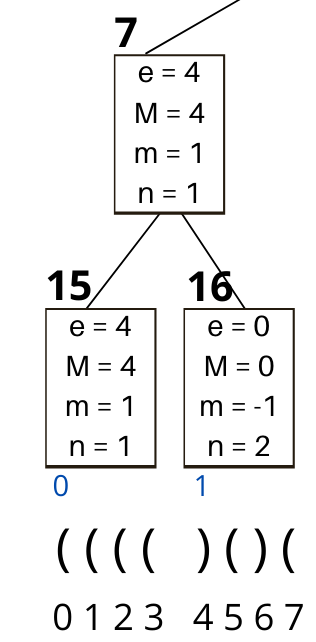
\includegraphics[scale=0.65]{images/internal-nodo.png}
        \end{minipage}
        \begin{minipage}[c]{0.49\linewidth}
            \begin{tabular}{l}\\
                R[7].e = R[15].e +  R[16].e.             \\
                R[7].M=max(R[15].M, R[15].e+ R[16].M).\\
                R[7].m=min(R[15].m, R[15].e+ R[16].m). \\
                R[7].n= R[15].n. \\
            \end{tabular}
        \end{minipage}
    \end{figure}
\end{frame}

\begin{frame}{rmM-tree: Operações}
    \begin{table}[]
       \begin{tabular}{|c|c|c|}
            \hline
            \multicolumn{3}{|c|}{\textbf{Operações}}  \\ \hline  
            fwdsearch(i,d)                       &bwdsearch(i,d)                        &minExcess(i,j) \\ \hline               
            maxExcess(i,j)                       & minSelectExcess(i,j,t)               & minCount(i,j)                       \\ \hline
            enclose(i)                           & rank\_v(i)                           & select\_v(i)                         \\ \hline                                
            findClose(i)                         & findOpen(i)                          & rmq(i,j) \\ \hline
            inspect(i)                           & preRank(i)                           & postRank(i)                    \\ \hline
            preSelect(i)                         & postSelect(i)                        & isLeaf(i)                       \\ \hline
            isAncestor(i,j)                      & depth(i)                             & parent(i)   \\ \hline
        \end{tabular}
    \end{table}
\end{frame}

\begin{frame}{rmM-tree: Operações}
    \begin{table}[]
        \begin{tabular}{|c|c|c|}
        \hline
        \multicolumn{3}{|c|}{\textbf{Operações}}                                                         \\ \hline
        firstChild(i) &  lastChild(i) & nextSibling(i) \\ \hline
        prevSibling(i)    & subtreeSize(i)                   & levelAncestor(i,d)         \\ \hline
        \multicolumn{1}{|c|}{level-next(i)} & levelPrev(i)  & \multicolumn{1}{c|}{levelLmost(d)} \\ \hline
        levelRmost(d)                      & lca(i,j)       & deepestNode(i)                     \\ \hline
        degree(i)                           & child(i,q)     & childRank(i)                       \\ \hline
        leafRank(i)                        & leafSelect(i) & lmostLeaf(i)                       \\ \hline
        \end{tabular}
    \end{table}
\end{frame}


\begin{frame}{rmM-tree: operações}
    Problema: Dado um nó codificado em $i=1$, encontrar o nó codificado em $j>i$, mais à esquerda de $i$.

    Solução: 
    $$nextSibling(i) = findClose(i) +1$$ 
    $$findClose(i) = fwdSearch(i,-1)$$ 
 \end{frame}

 \begin{frame}{rmM-tree: $nextSibling$}
    Problema: Computar $nextSibling(1)$.
     \begin{figure}[h!]
         \centering
         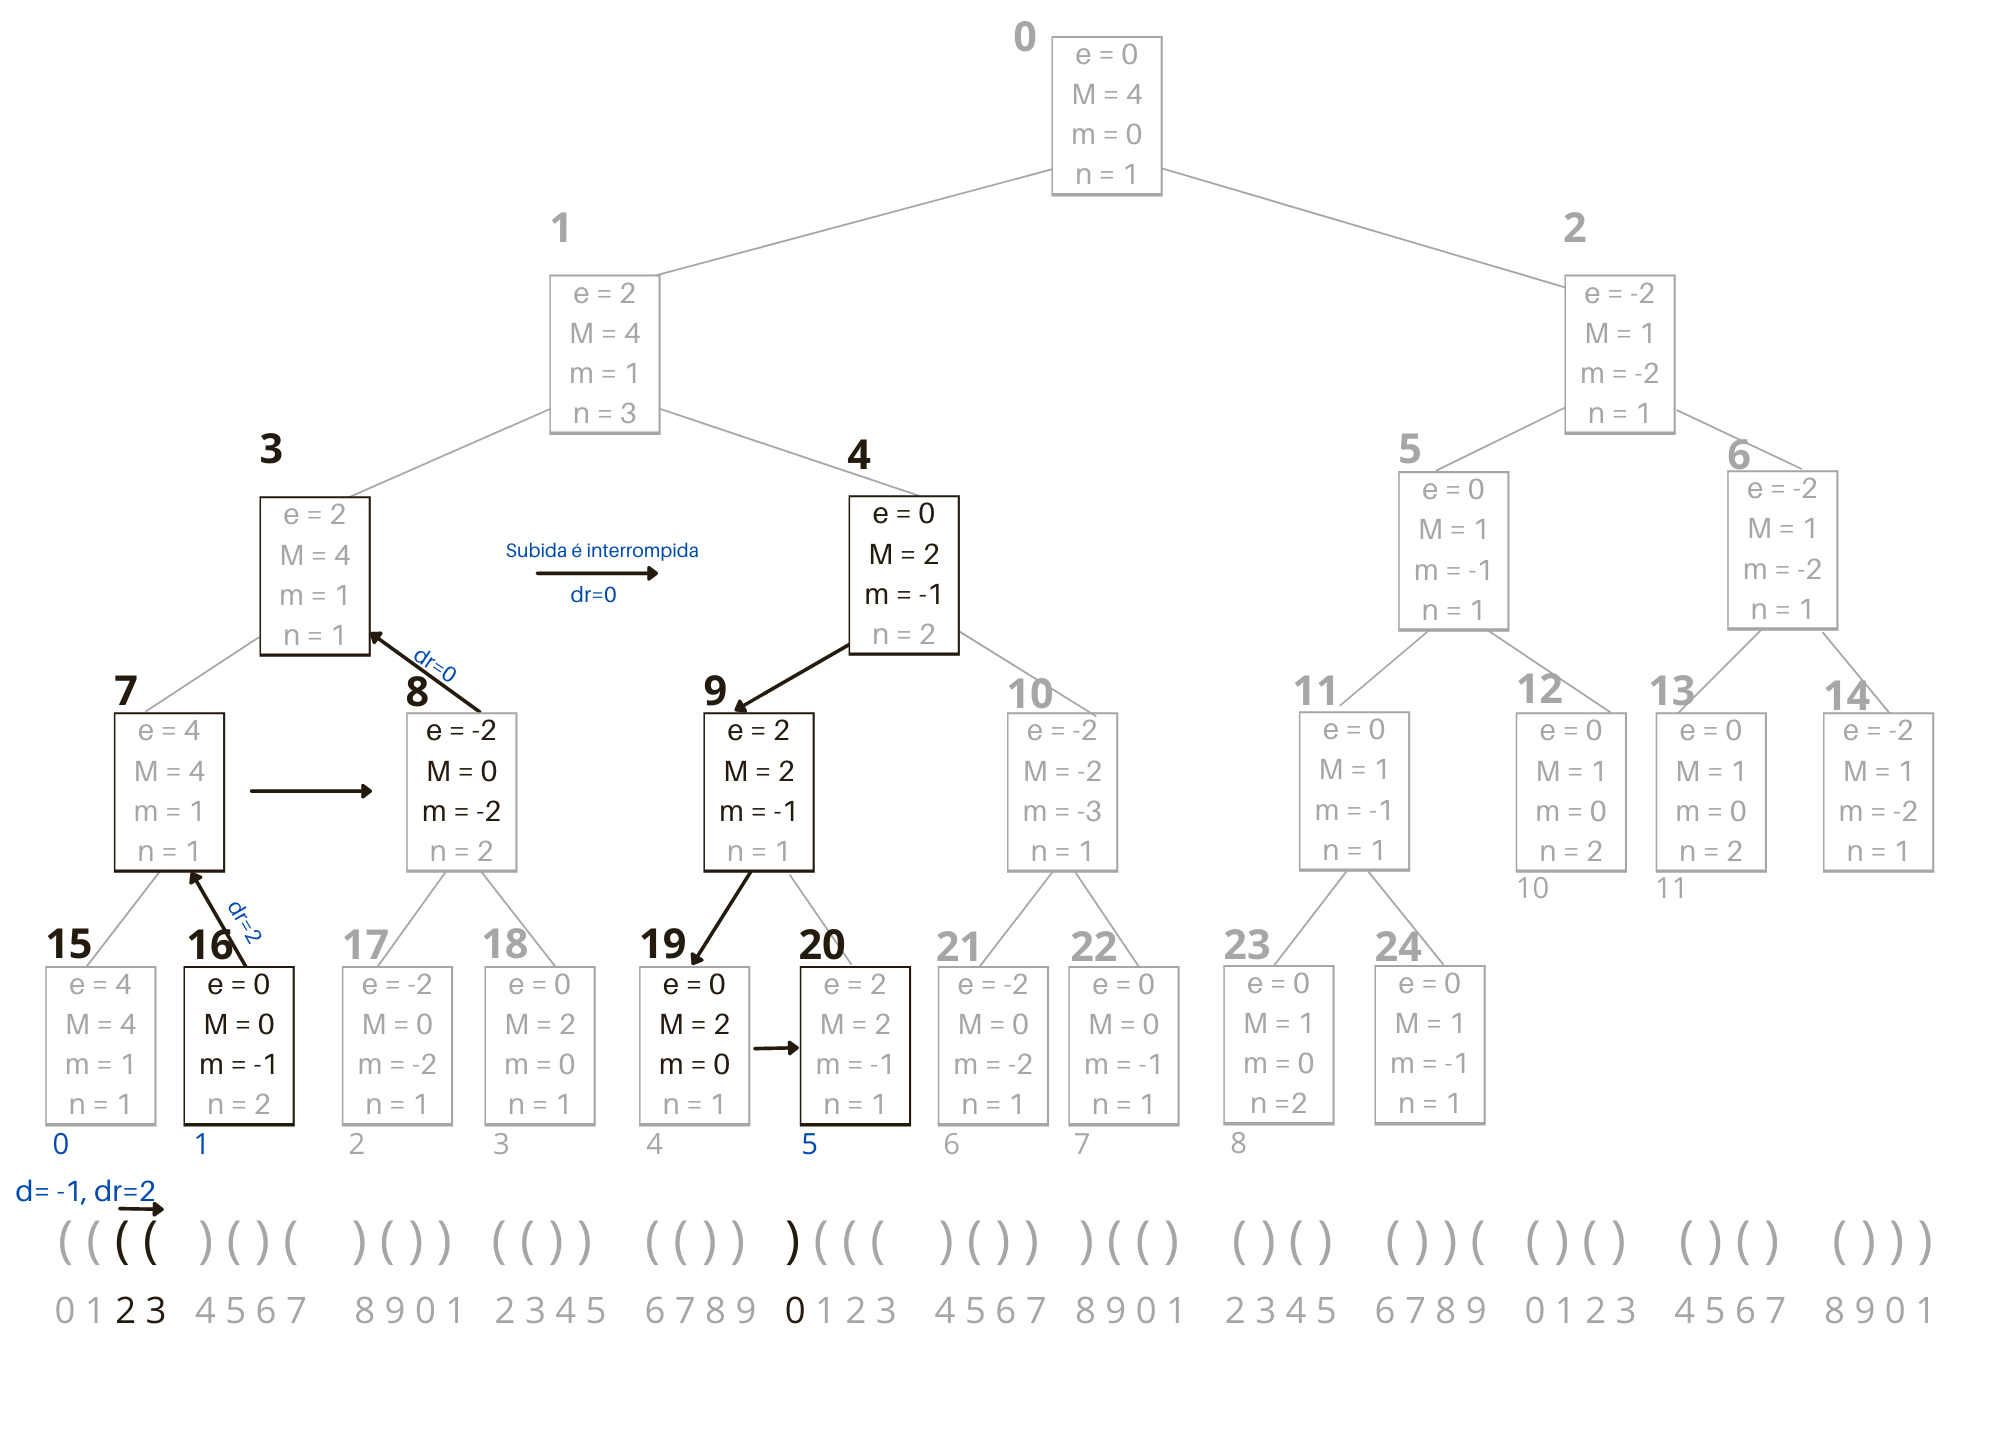
\includegraphics[scale=0.27]{images/rmm-tree-bin-fwdSearch.png}\\
         \caption{Simulação de $fwdSearch(1,-1)=20$}
     \end{figure} 
 \end{frame}

 \begin{frame}{rmM-tree: $nextSibling$}
    Problema: Dado um nó codificado em $i=1$, encontrar o nó codificado em $j>i$, mais à esquerda de $i$.

    Solução: 
    $$findClose(1) = fwdSearch(1,-1) = 20 $$ 
    $$nextSibling(1) = fwdSearch(1,-1) + 1 = 21 $$ 
 \end{frame}

 \begin{frame}{rmM-tree: $nextSibling$}
    Solução:  $nextSibling(1)$.
     \begin{figure}[h!]
         \centering
         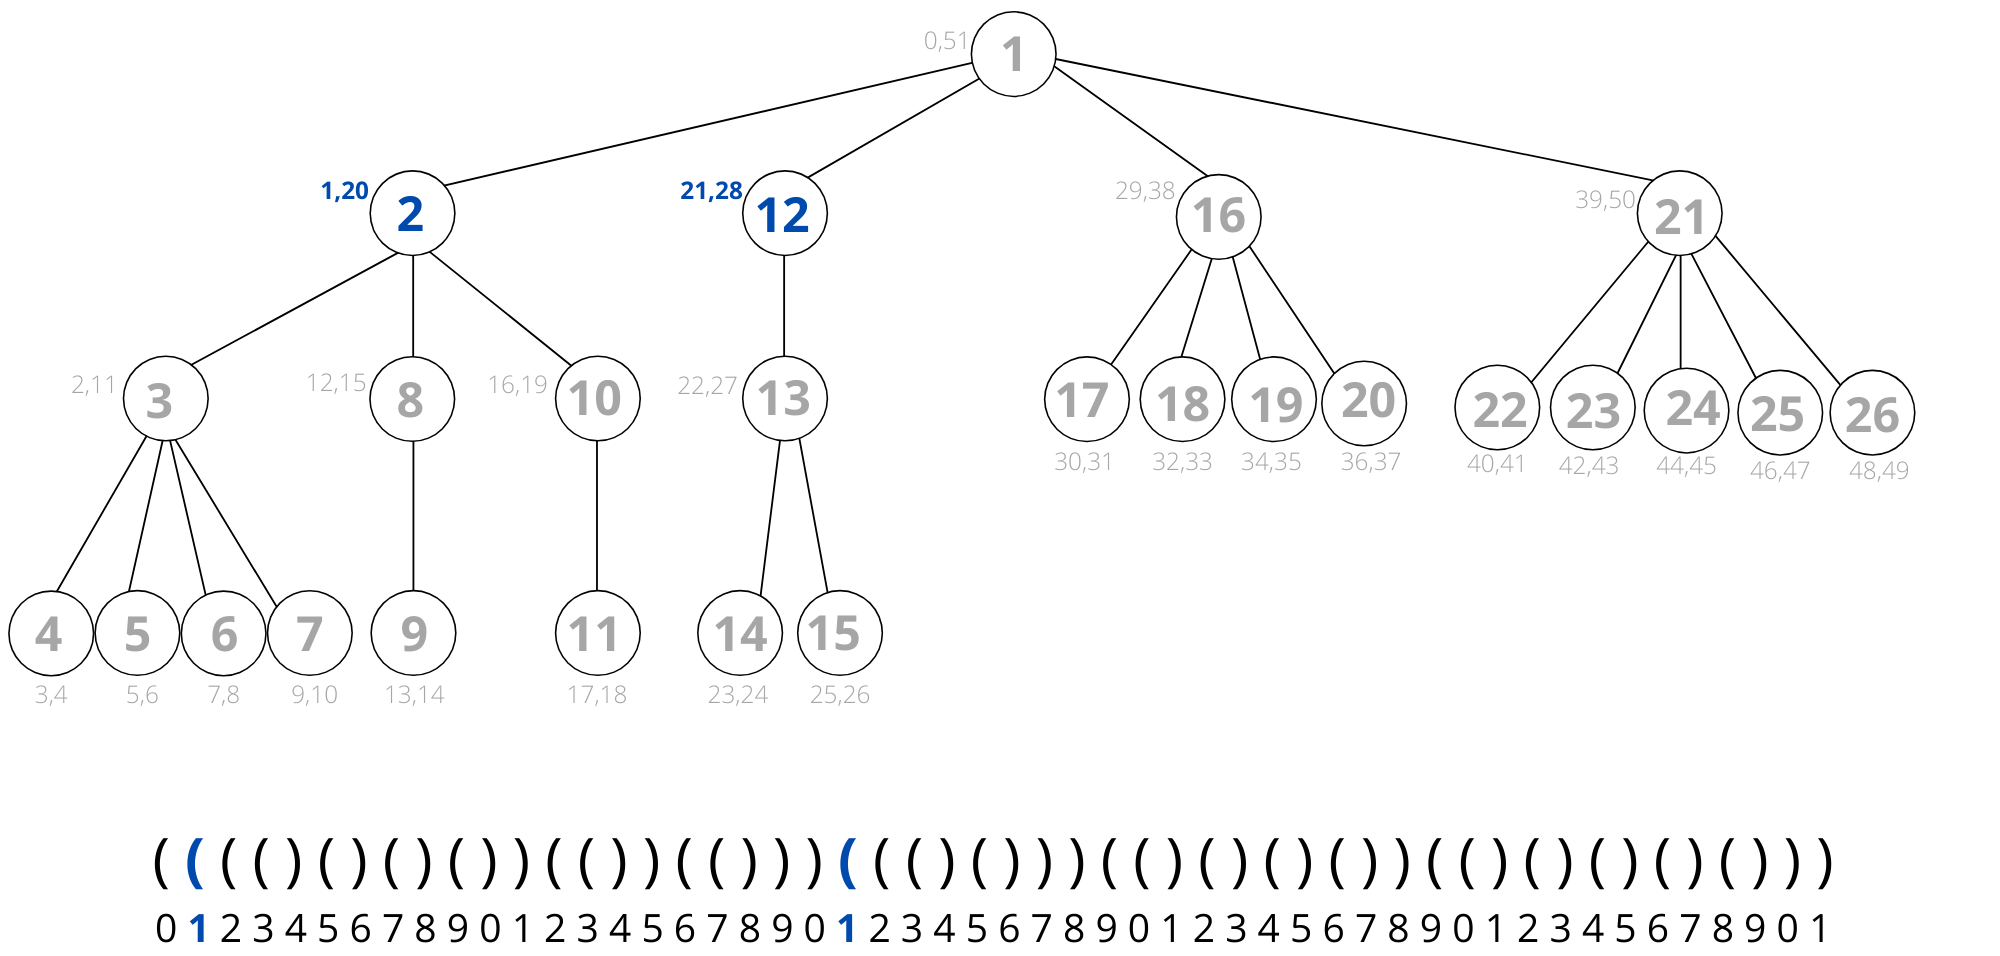
\includegraphics[scale=0.40]{images/nextSibling-res.png}\\
         \caption{Árvore de entrada}
     \end{figure} 
 \end{frame}

\begin{frame}{rmM-tree: operações}
    Problema: Verificar o ancestral comum mais baixo dos nós codificados em $i=5$ e $j=17$.
     \begin{figure}[h!]
         \centering
         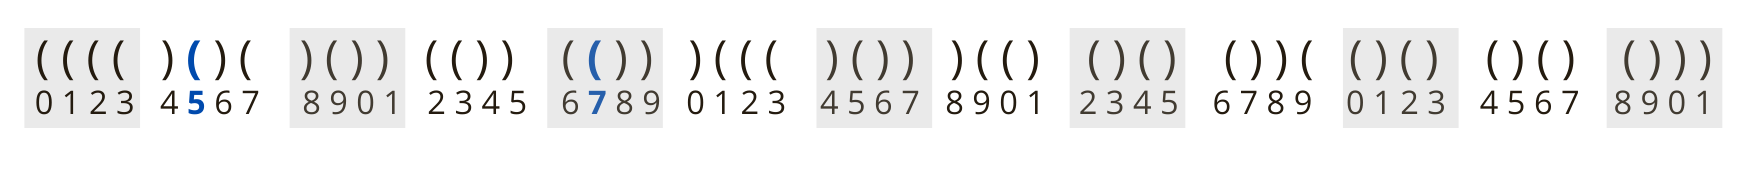
\includegraphics[scale=0.7]{images/bp-sequence.png}\\
         \caption{Sequência de parênteses balanceados, representando uma árvore $T$}
     \end{figure} 
 
 \end{frame}

 \begin{frame}{rmM-tree: $lca$}
    Problema: Verificar o ancestral comum mais baixo dos nós codificados em $i=5$ e $j=17$.

    Solução: 
    $$lca(i,j) = 
    \begin{cases}
          i,  \mbox{se } isAncestor(i,j); \\
         j, \mbox{se } isAncestor(j,i); \\
         parent(rmq(i ,j)+1)
    \end{cases}
    $$ 
 \end{frame}

 \begin{frame}{rmM-tree: $lca$}
    Problema: Verificar o ancestral comum (mais baixo) dos nós codificados em $i=5$ e $j=17$.


    Solução:\\
    \begin{itemize}
        \item \textit{isAncestor(,i,j)} verifica se o nó codificado em $i$ é ancestral do nó $j$;
        \item O mesmo vale para \textit{isAncestor(j,i)};
        \item Usar o terceiro caso.
    \end{itemize}
 \end{frame}


 \begin{frame}{rmM-tree: $lca$}
    Problema: Computar $lca(5,17)$.


    Solução: $ parent(rmq(i ,j)+1)$\\
    \begin{itemize}
        \item $rmq(i,j) = fwdSearch(i-1, minExcess(i,j))$;
        \item $parent(rmq(i,j)+1) = bwdSearch(rmq(i,j)+1, 0) + 1$.
    \end{itemize}
 \end{frame}


\begin{frame}{rmM-tree: $lca$}
    Problema: Computar $lca(5,17)$.
     \begin{figure}[h!]
         \centering
         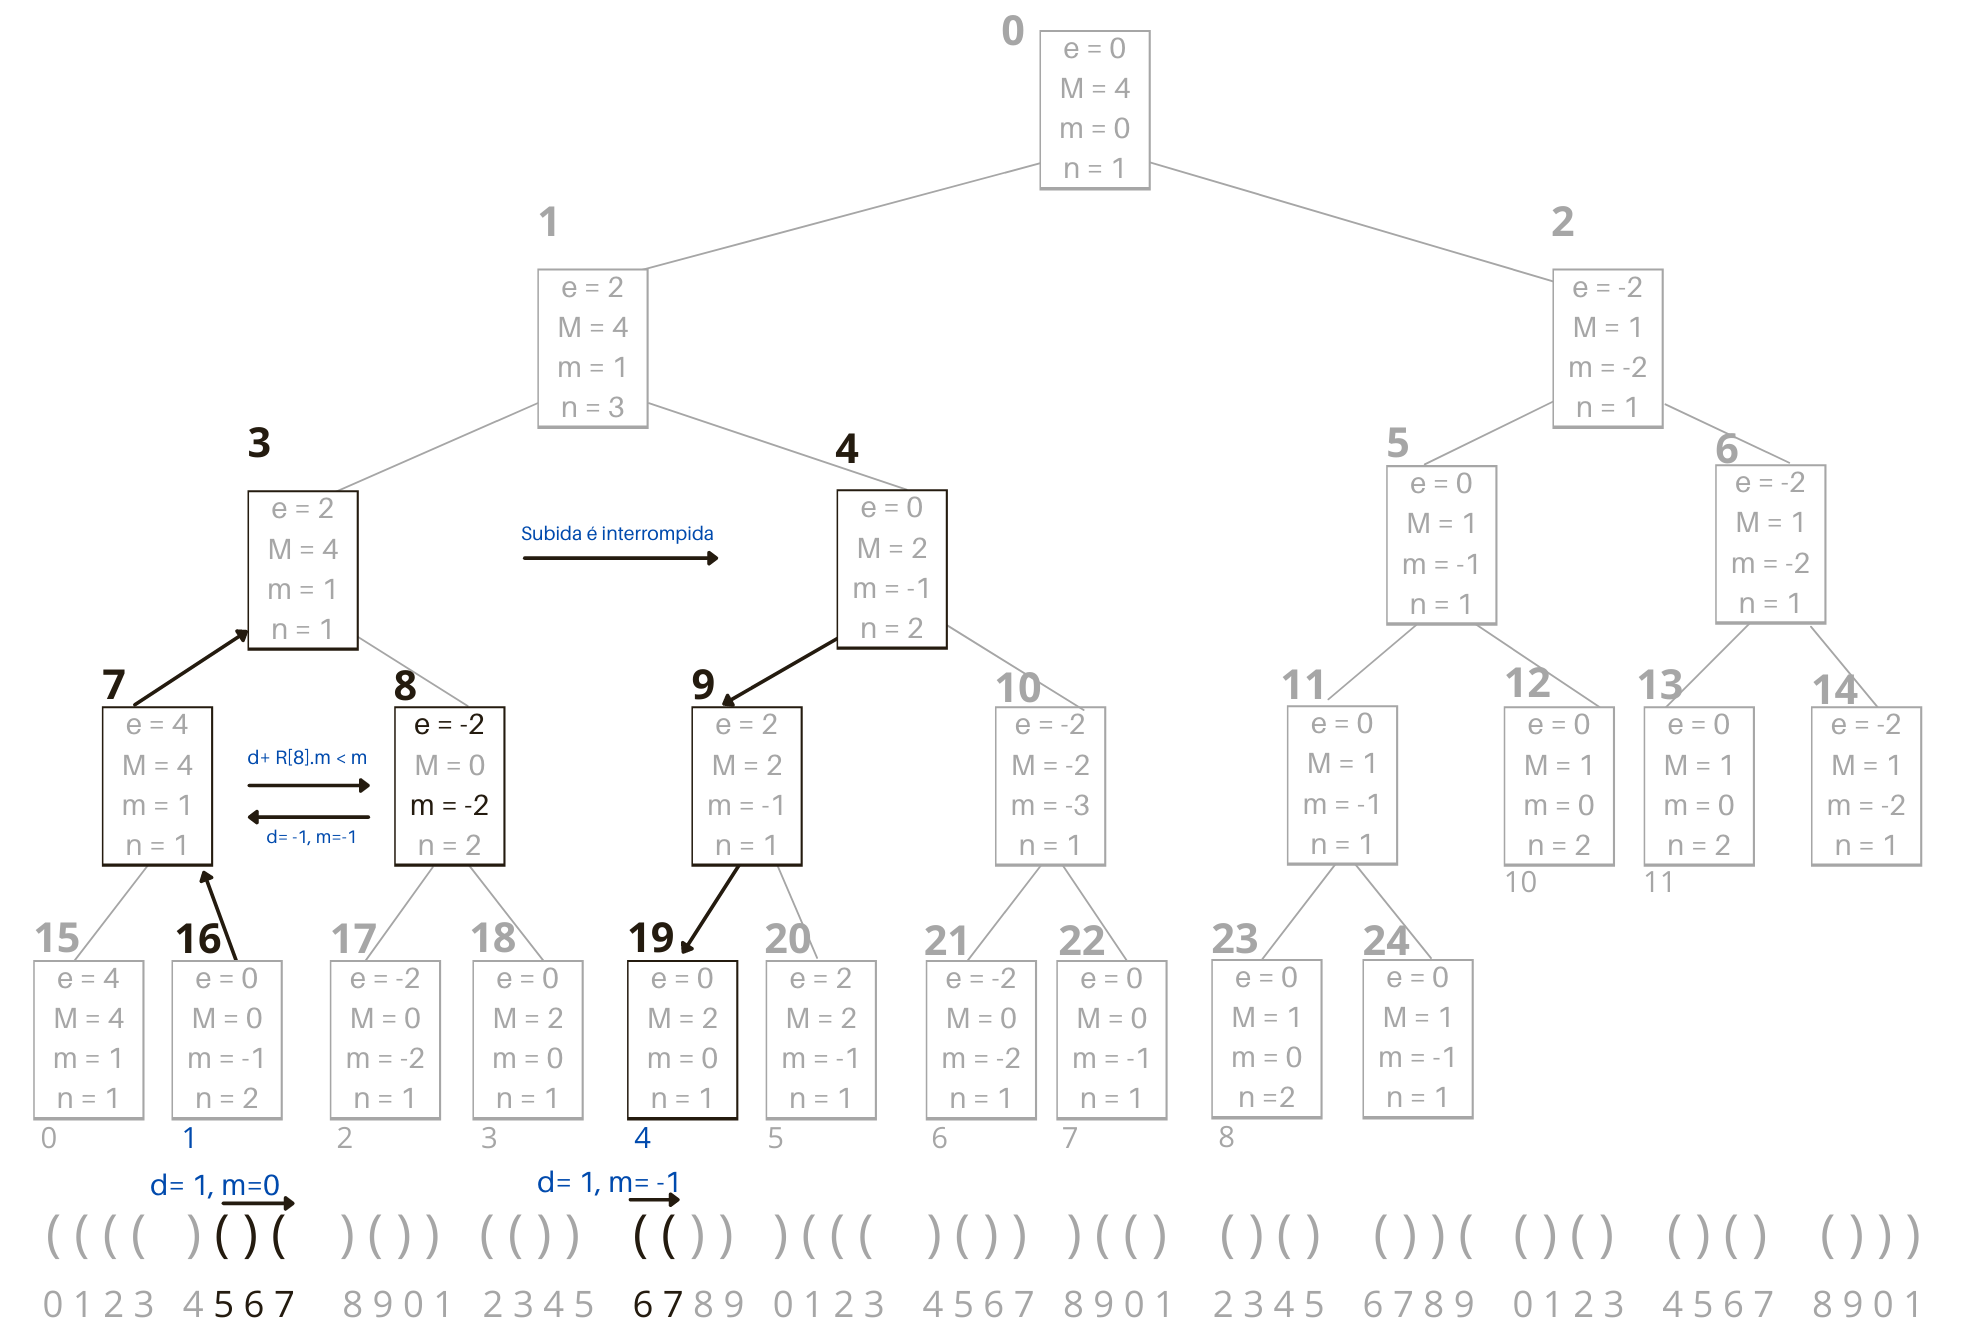
\includegraphics[scale=0.27]{images/rmm-tree-bin-minexcess.png}\\
         \caption{Simulação de $minExcess(5,17)=-1$}
     \end{figure} 
 \end{frame}


% \begin{frame}{rmM-tree: operações}
%     Problema: Computar $lca(5,17)$.
%      \begin{figure}[h!]
%          \centering
%          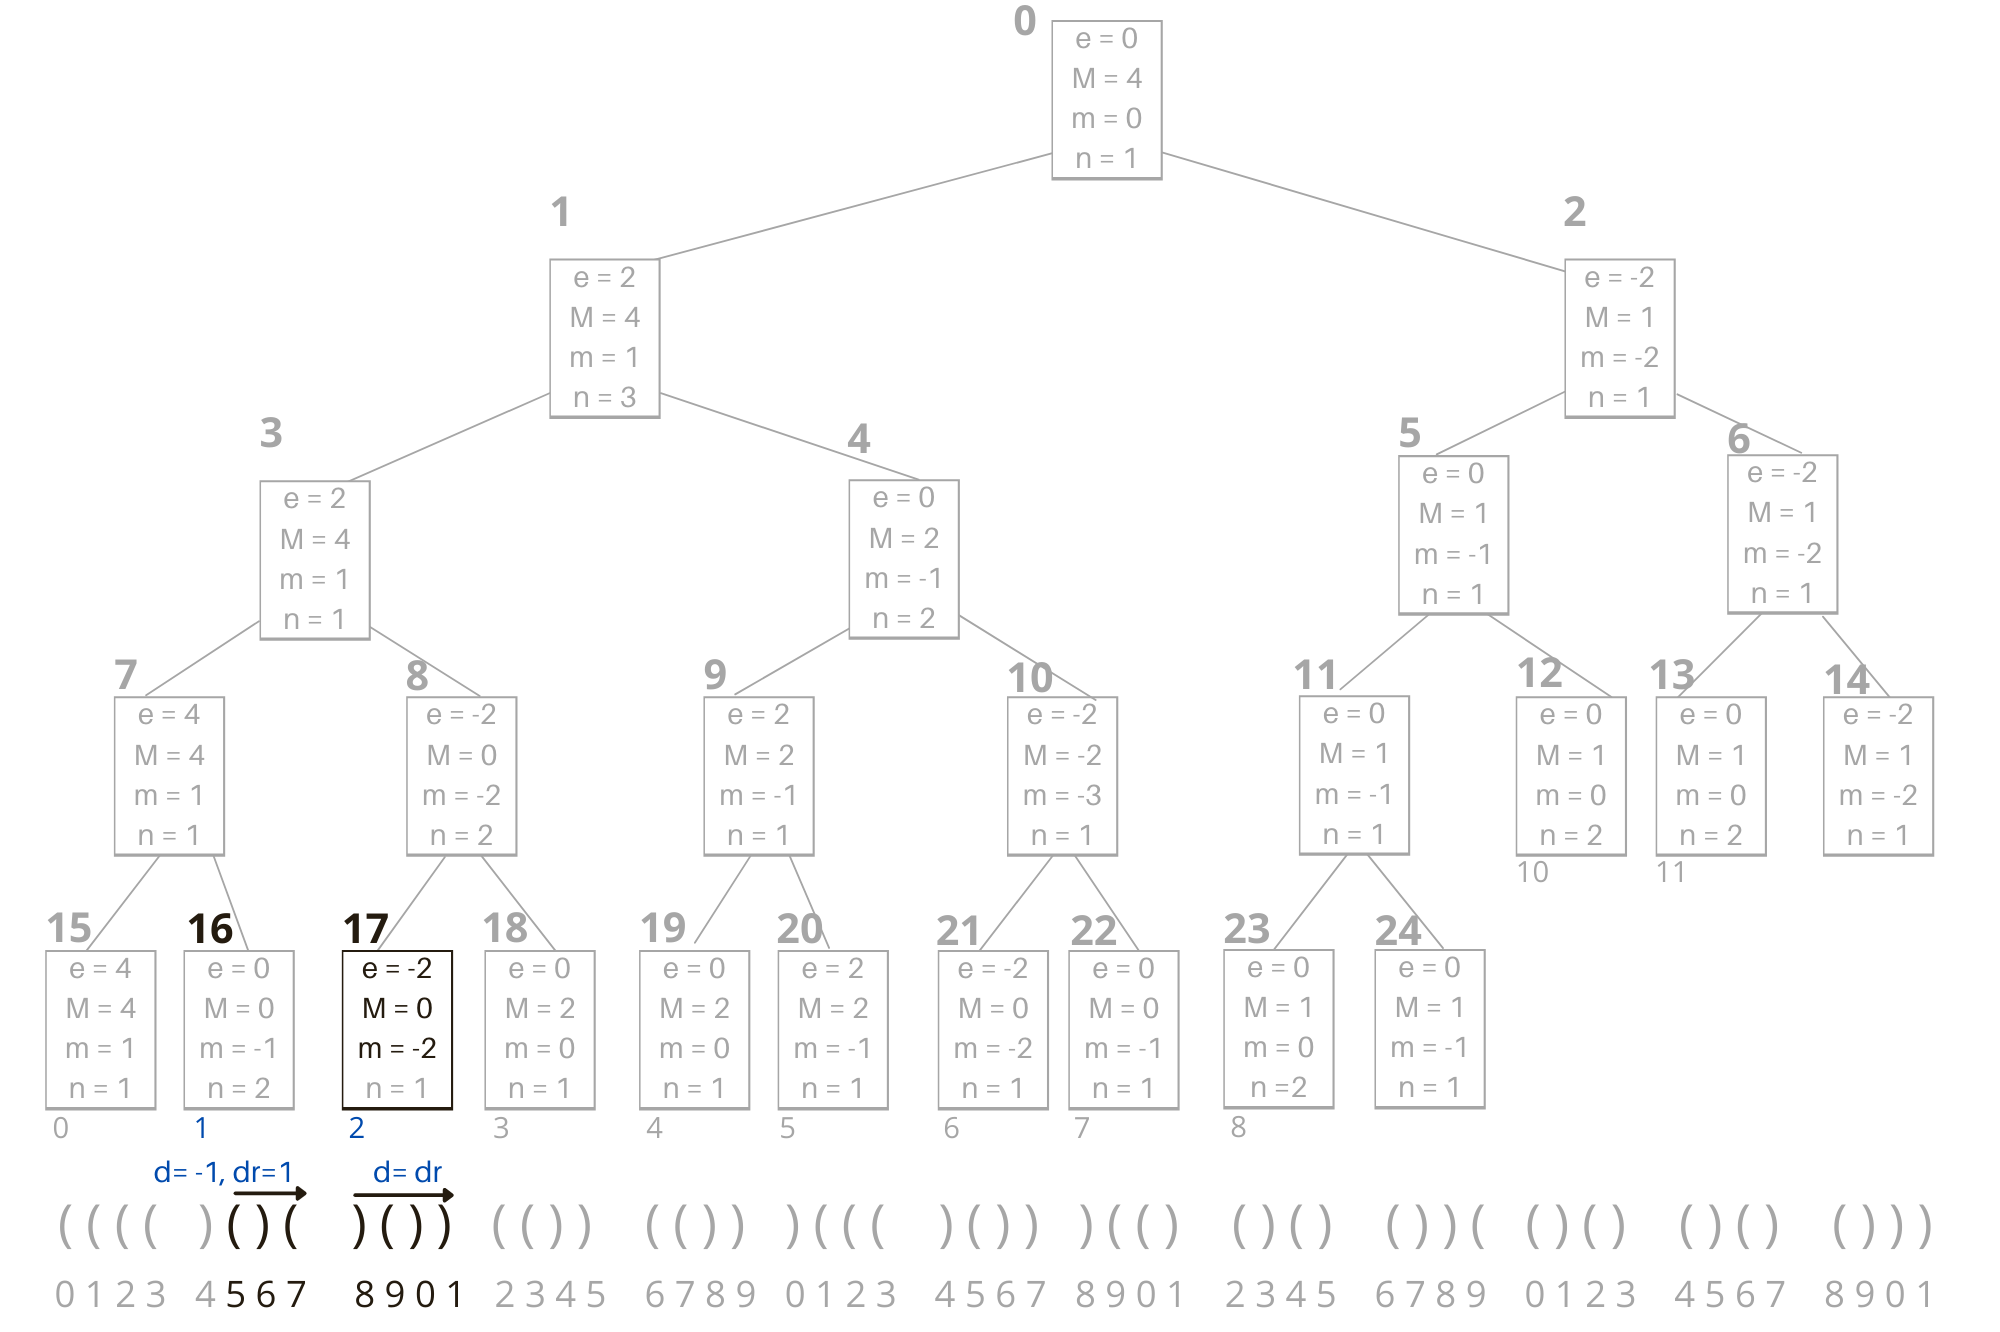
\includegraphics[scale=0.27]{images/rmm-tree-bin-fwd-lca.png}\\
%          \caption{Simulação de $fwdSearch(4,-1)=11$}
%      \end{figure} 
%  \end{frame}

 \begin{frame}{rmM-tree: $lca$}
    Solução: Computar $lca(5,17)$.
     \begin{figure}[h!]
         \centering
         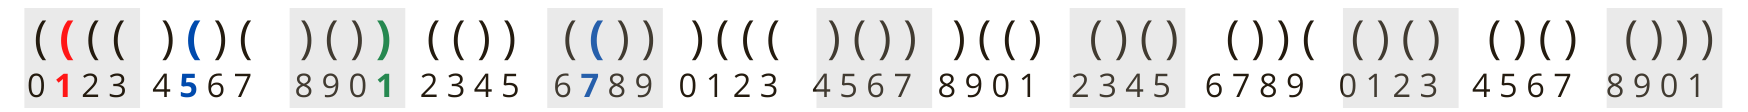
\includegraphics[scale=0.8]{images/lca-resposta.png}\\
         \caption{Nós acessados durante a operação $lca(5,17)$}
     \end{figure} 
 \end{frame}

 \begin{frame}{rmM-tree: $lca$}
    Solução: Computar $lca(5,17)$.
     \begin{figure}[h!]
         \centering
         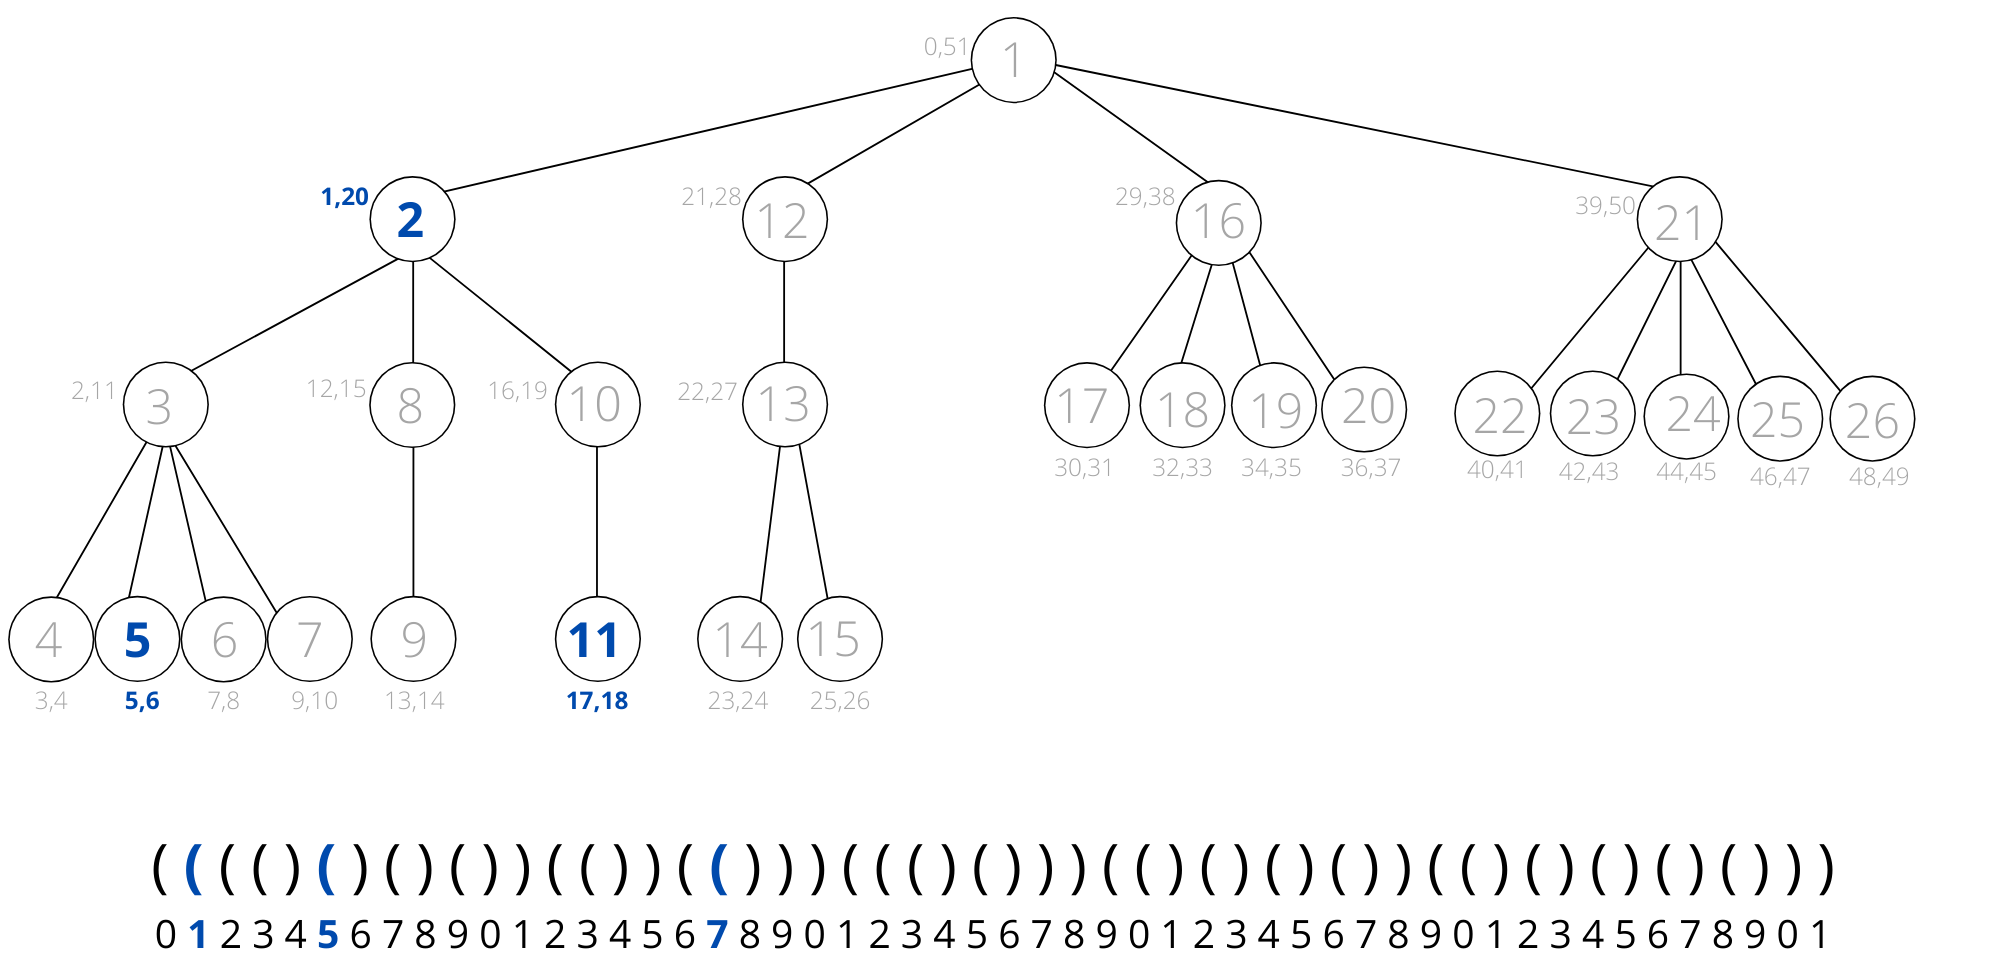
\includegraphics[scale=0.40]{images/lca-res.png}\\
         \caption{Árvore de entrada}
     \end{figure} 
 \end{frame}

\begin{frame}{Aproveitamento de cache}
    \begin{itemize}
        \item Expansão da memória principal;
        \item Dados residindo em memória principal: um novo gargalo;
        \item Falhas de cache.
    \end{itemize}
\end{frame}

\begin{frame}{Aproveitamento de cache}
    \begin{itemize}
        \item Maximização da quantidade de informação em um nó \cite{paper-effect-node-size-cache-b-trees}:
        \begin{itemize}
            \item Altura da árvore;
            \item Linha de cache.
        \end{itemize}
        \item Fator de ramificação \cite{paper-making-btree-cache}:
        \begin{itemize}
            \item Cache Sensitive Tree (CSS-tree);
            \item Cache Sensitive B$^+$-Tree (CS$B^+$-tree);
            \item Árvores B$^+$.
        \end{itemize}
    \end{itemize}
\end{frame}
\section{Proposta}

\begin{frame}{range min-Max tree k-ária (rmM-tree k-ária)}
    Características:
        \begin{itemize}
            \item Alto fator de ramificação;
            \item Maior cobertura de área por nó;
            \item Cada nó cobre até $k$ intervalos;
            \item Mesmas definições de registros da estrutura binária;
            \item Complexidade de tempo e espaço eficientes, usando os mesmos campos defindos por \cite{book-compact-data-structures} em sua estrutura.
        \end{itemize}
\end{frame}

\begin{frame}{rmM-tree k-ária}
    \textbf{Árvore de entrada}
        \begin{figure}[h!]
            \centering
            
            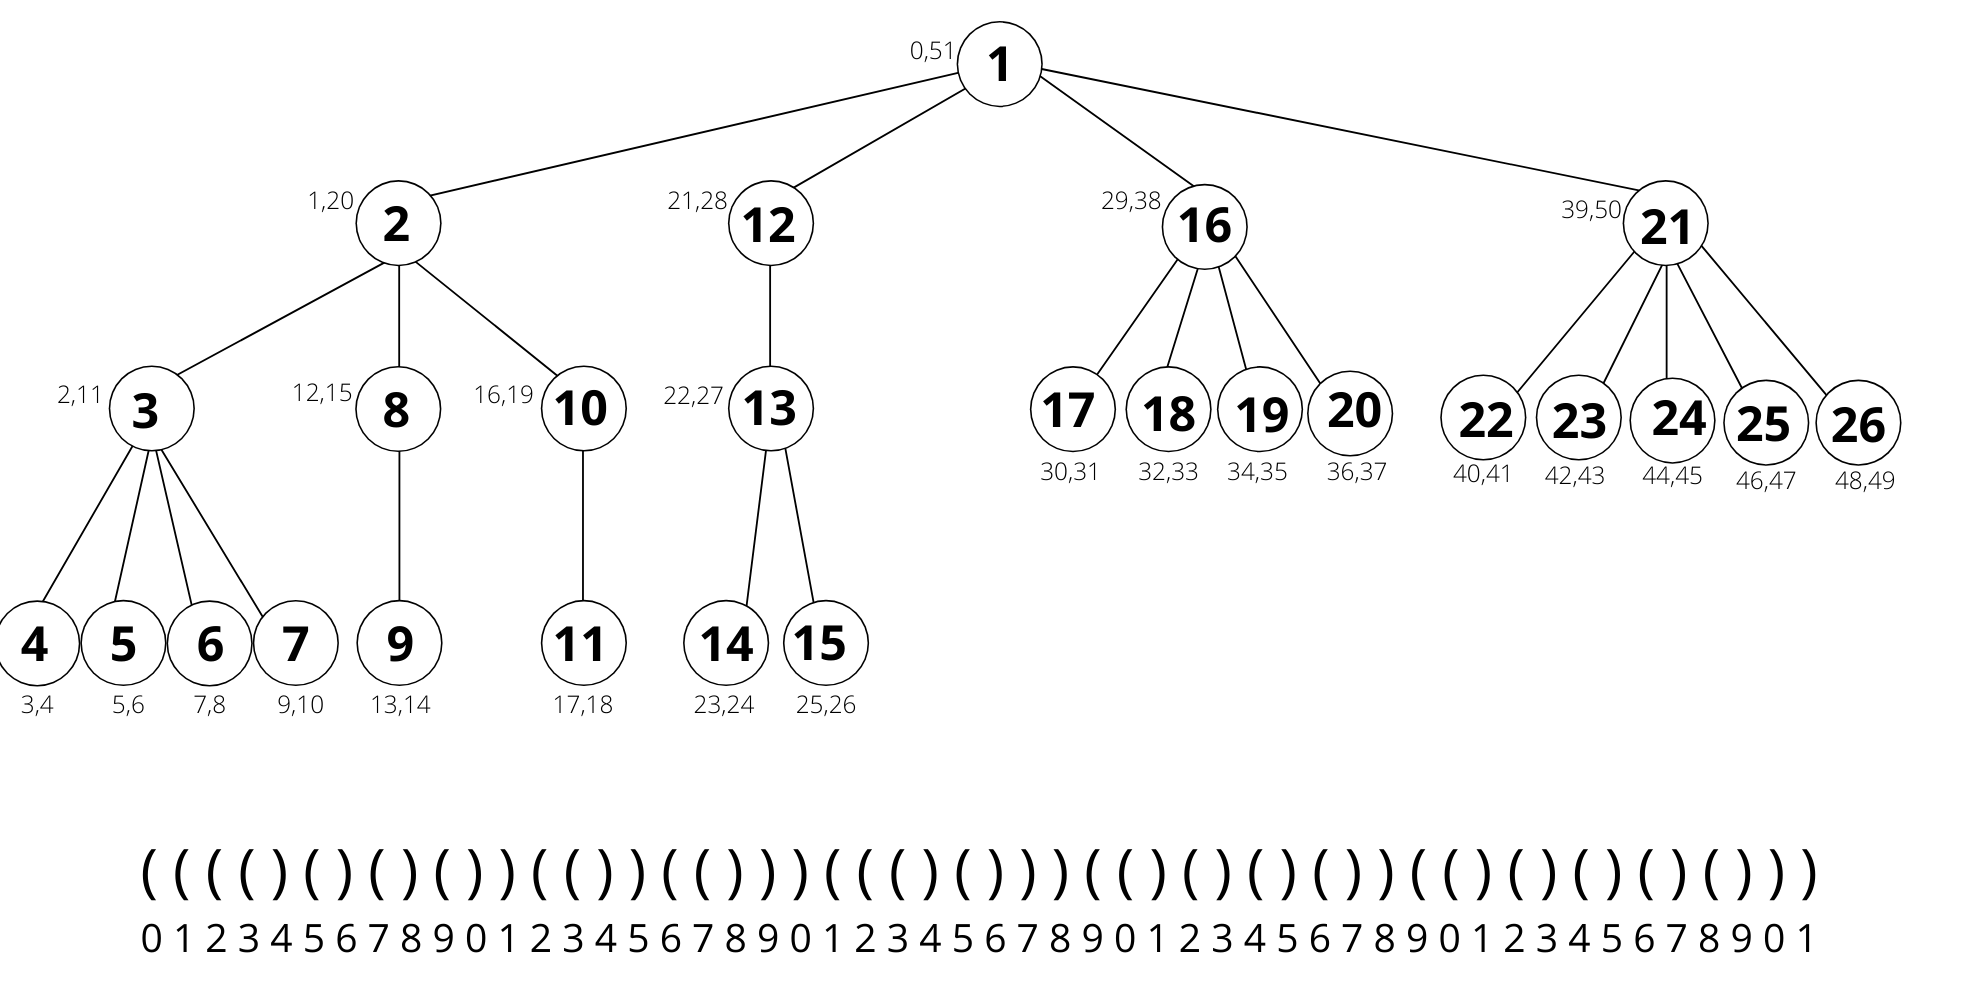
\includegraphics[scale=0.37]{images/arvore_geral.png}
        \end{figure} 
\end{frame}

\begin{frame}{rmM-tree k-ária: Registros}
    \begin{figure}[h!]
        \centering
        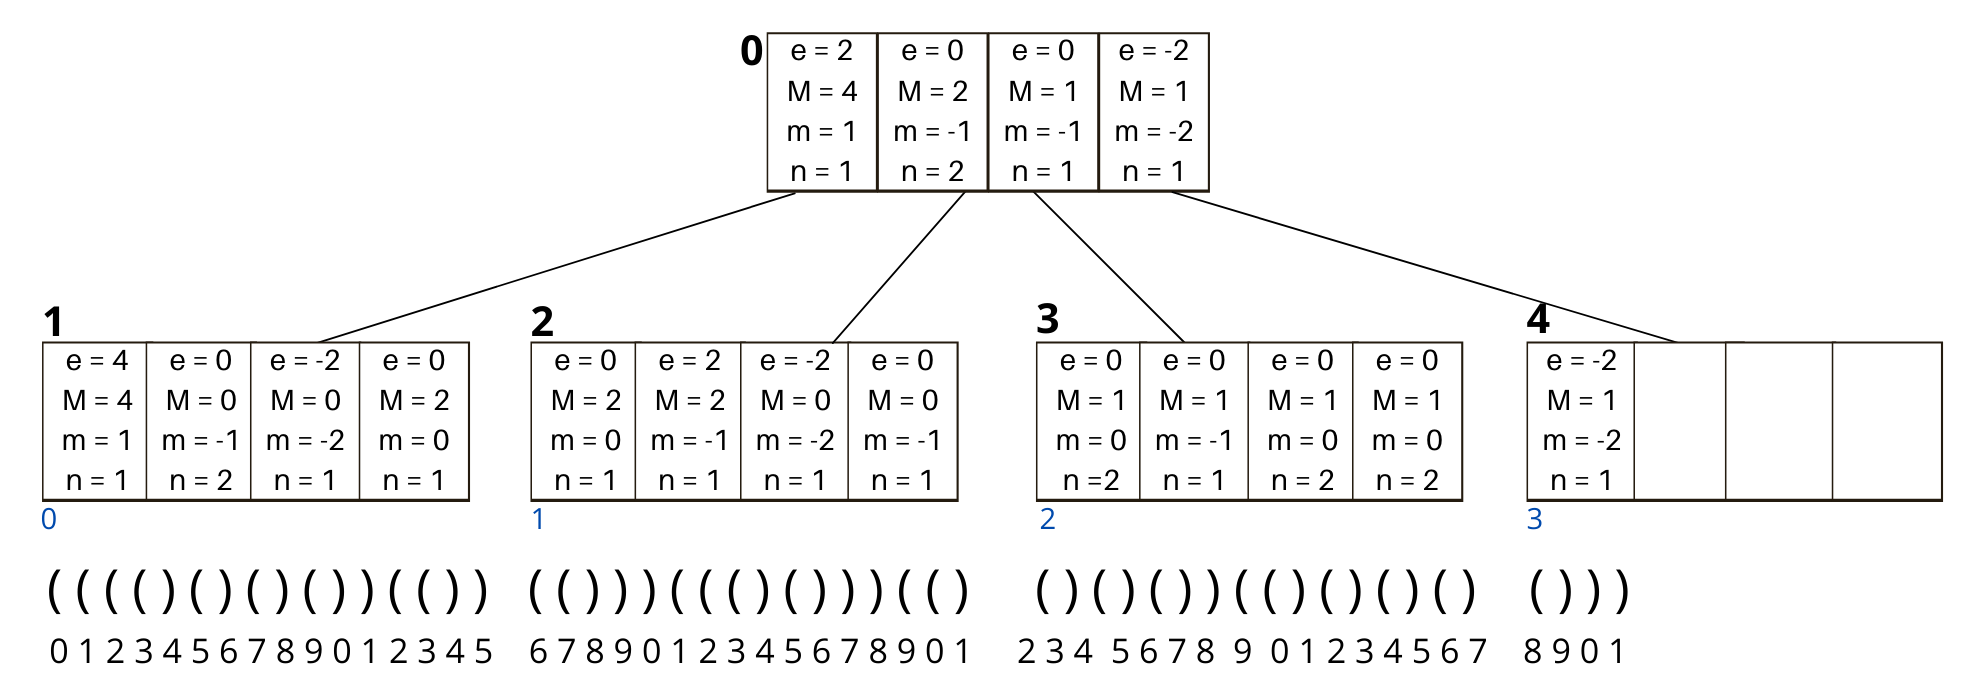
\includegraphics[scale=0.4]{images/rmm-tree-kary.png}\\
        \caption{rmM-tree 4-ária com blocos de tamanho 4}
    \end{figure} 
\end{frame}

\begin{frame}{rmM-tree k-ária: Registros}
    \textbf{Nós internos e raíz}
    \begin{figure}[h]
        \begin{minipage}[c]{0.25\linewidth}
            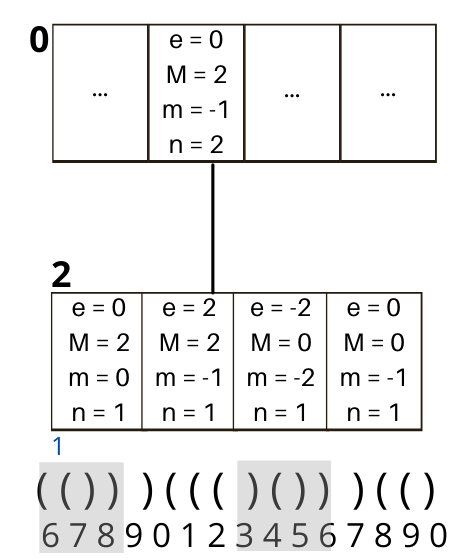
\includegraphics[scale=0.70]{images/k-internal-nodes.png}
        \end{minipage}
        \begin{minipage}[c]{0.70\linewidth}
                \begin{eqnarray*}
                    \begin{split}
                        R[0][1].M =& max(R[2][0].M, \\
                        &   R[2][0].e + R[2][1].M, \\
                        &   R[2][0].e + R[2][1].e + R[2][2].M,  \\
                        &   R[2][0].e + R[2][1].e + R[2][2].e  +\\
                        &   R[2][3].M)\\
                        &   = max(2,2,2,0) = 2;
                    \end{split}
                \end{eqnarray*}
        \end{minipage}
    \end{figure}
\end{frame}

\begin{frame}{rmM-tree k-ary: Operações}
    \begin{table}
        \centering
        \caption[Operações sobre a rmM-tree binária e k-ária]{Operações suportadas pela rmM-tree binária e rmM-tree-kária}
	    \resizebox{\columnwidth}{!}{
            \begin{tabular}{|c|c|c|}
                \hline
                \textbf{Operação} & \textbf{rmM-tree binária} & \textbf{rmM-tree k-ária}\\ \hline
                fwdSearch(i,d)  &  \cmark \par &   \cmark \par\\ \hline
                bwdSearch(i,d)  &  \cmark \par &   \cmark \par\\ \hline
                minExcess(i,j) / maxExcess(i,j)  &   \cmark \par & \xmark \\ \hline
                minCount(i,j)  &   \cmark \par & \xmark\\ \hline
                minSelectExcess(i,j,t)  &  \cmark \par & \xmark\\ \hline
                enclose(i) &  \cmark \par &   \cmark \par \\ \hline
                rmq(i,j) / rMq(i,j) &  \cmark \par & \xmark \\ \hline
                rank$_1$(i) / rank$_0$(i) &  \cmark \par &    \cmark \par\\ \hline
                select$_1$(i) / select$_0$(i) &  \cmark \par &   \cmark \par\\ \hline
            \end{tabular}
        }
    \end{table}
\end{frame}

\begin{frame}{rmM-tree k-ary: Operações}
    \begin{table}
        \centering
        \caption[Operações sobre a rmM-tree binária e k-ária]{Operações suportadas pela rmM-tree binária e rmM-tree-kária}
	    \resizebox{\columnwidth}{!}{
            \begin{tabular}{|c|c|c|}
                \hline
                \textbf{Operação} & \textbf{rmM-tree binária} & \textbf{rmM-tree k-ária}\\ \hline
                preRank(i)/postRank(i) &  \cmark \par &   \cmark \par\\ \hline
                preSelect(i)/postSelect(i) &  \cmark \par &   \cmark \par \\ \hline
                isLeaf(i) &  \cmark \par &   \cmark \par\\ \hline
                isAncestor(i,j) &  \cmark \par &   \cmark \par\\ \hline
                depth(i) &   \cmark \par &   \cmark \par\\ \hline
                parent(i) &  \cmark \par &   \cmark \par\\ \hline
                firstChild(i) / lastChild(i) &  \cmark \par &   \cmark \par\\ \hline
                child(i,t)&  \cmark \par & \xmark \\ \hline
                nextSibling(i) / prevSibling(i) &   \cmark \par &   \cmark \par\\ \hline
            \end{tabular}
        }
    \end{table}
\end{frame}

\begin{frame}{rmM-tree k-ary: Operações}
    \begin{table}
        \centering
        \caption[Operações sobre a rmM-tree binária e k-ária]{Operações suportadas pela rmM-tree binária e rmM-tree-kária}
	    \resizebox{\columnwidth}{!}{
            \begin{tabular}{|c|c|c|}
                \hline
                \textbf{Operação} & \textbf{rmM-tree binária} & \textbf{rmM-tree k-ária}\\ \hline
                subtreeSize(i) &   \cmark \par &   \cmark \par\\ \hline
                levelAncestor(i,d) &   \cmark \par &   \cmark \par \\ \hline
                levelNext(i) / levelPrev(i) &   \cmark \par &   \cmark \par \\ \hline
                levelLeftMost(d) / levelRightMost(d) &  \cmark \par &   \cmark \par\\ \hline
                lca(i,j)&  \cmark \par & \xmark\\ \hline
                deepestNode(i)&  \cmark \par & \xmark \\ \hline
                degree(i)&  \cmark \par & \xmark\\ \hline
                childRank(i)&  \cmark \par & \xmark\\ \hline
                leafRank(i)/leafSelect(i)&  \cmark \par  &   \cmark \par\\ \hline
                leftMostLeaf(i)/rightMostLeaf(i)&   \cmark \par &   \cmark \par\\ \hline
            \end{tabular}
        }
    \end{table}
\end{frame}


\begin{frame}{rmM-tree k-ary: operações}
    Problema: Dado um nó codificado em $i=1$, encontrar o nó codificado em $j>i$, mais à esquerda de $i$.

    Solução: 
    $$nextSibling(i) = findClose(i) +1$$ 
    $$findClose(i) = fwdSearch(i,-1)$$ 
 \end{frame}

 \begin{frame}{rmM-tree k-ary: $nextSibling$}
    Problema: Computar $nextSibling(1)$.
     \begin{figure}[h!]
         \centering
         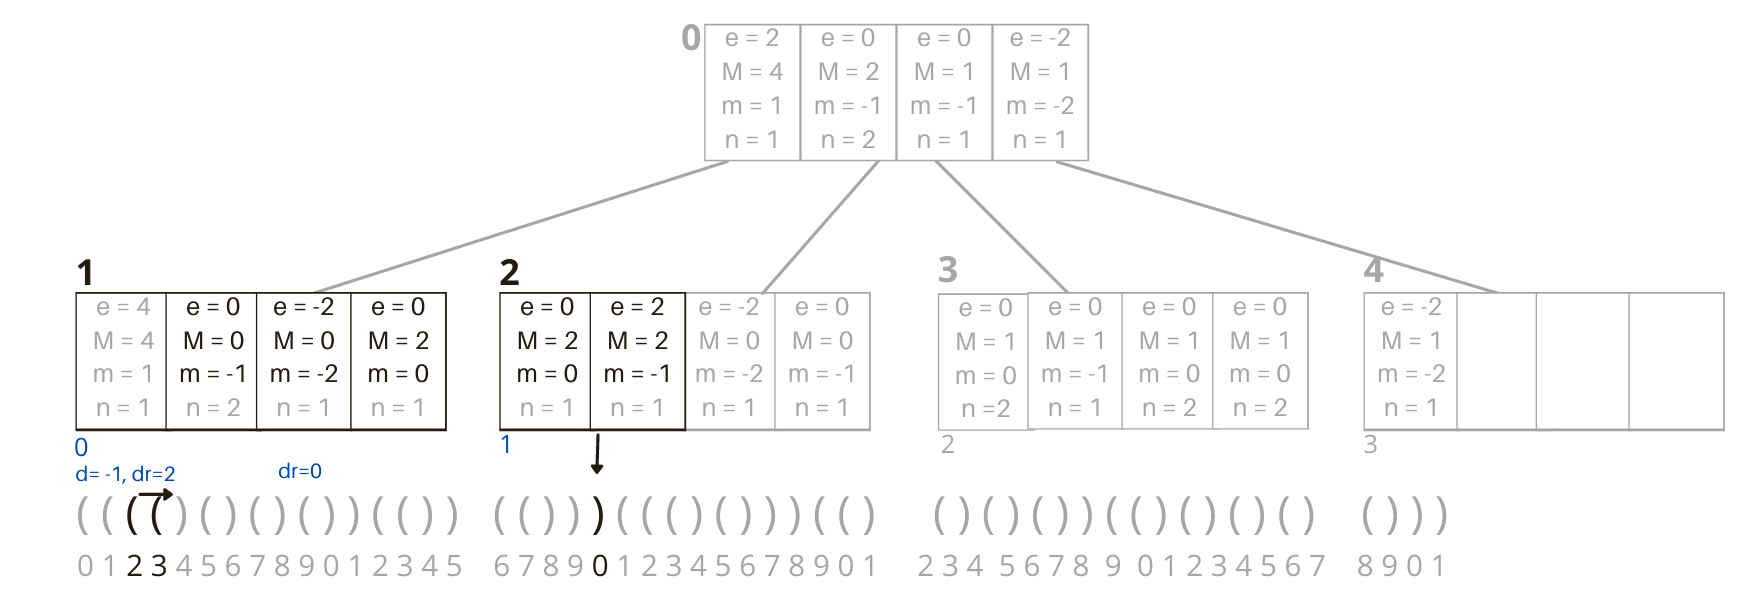
\includegraphics[scale=0.8]{images/rmm-tree-kary-fwd.png}\\
         \caption{Simulação de $fwdSearch(1,-1)=20$ em uma rmM-tree 4-ária}
     \end{figure} 
 \end{frame}


 \begin{frame}{rmM-tree k-ary: $nextSibling$}
    Problema: Dado um nó codificado em $i=1$, encontrar o nó codificado em $j>i$, mais à esquerda de $i$.

    Solução: 
    $$findClose(1) = fwdSearch(1,-1) = 20 $$ 
    $$nextSibling(1) = fwdSearch(1,-1) + 1 = 21 $$ 
 \end{frame}

 \begin{frame}{rmM-tree k-ary: $nextSibling$}
    Solução:  $nextSibling(1)$.
     \begin{figure}[h!]
         \centering
         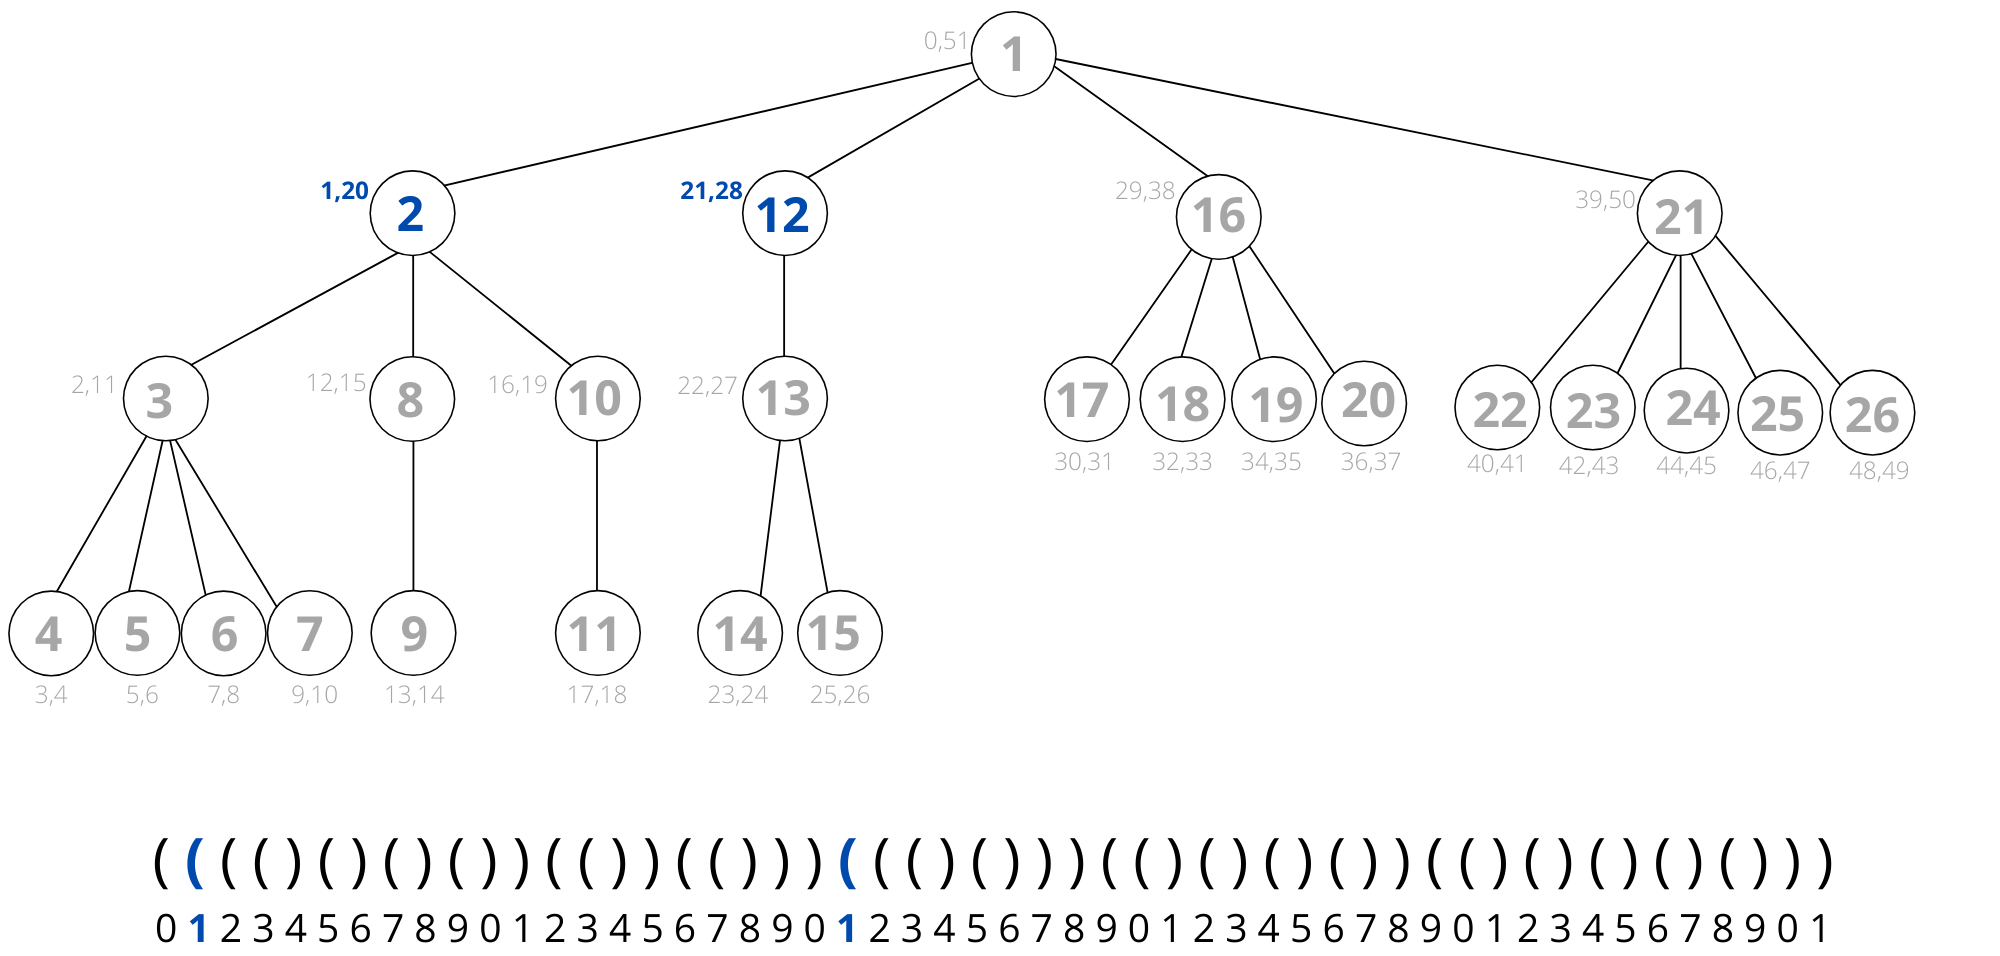
\includegraphics[scale=0.40]{images/nextSibling-res.png}\\
         \caption{Árvore de entrada}
     \end{figure} 
 \end{frame}

 \begin{frame}{rmM-tree k-ary: $nextSibling$}
    Problema: Computar $nextSibling(1)$.
     \begin{figure}[h!]
         \centering
         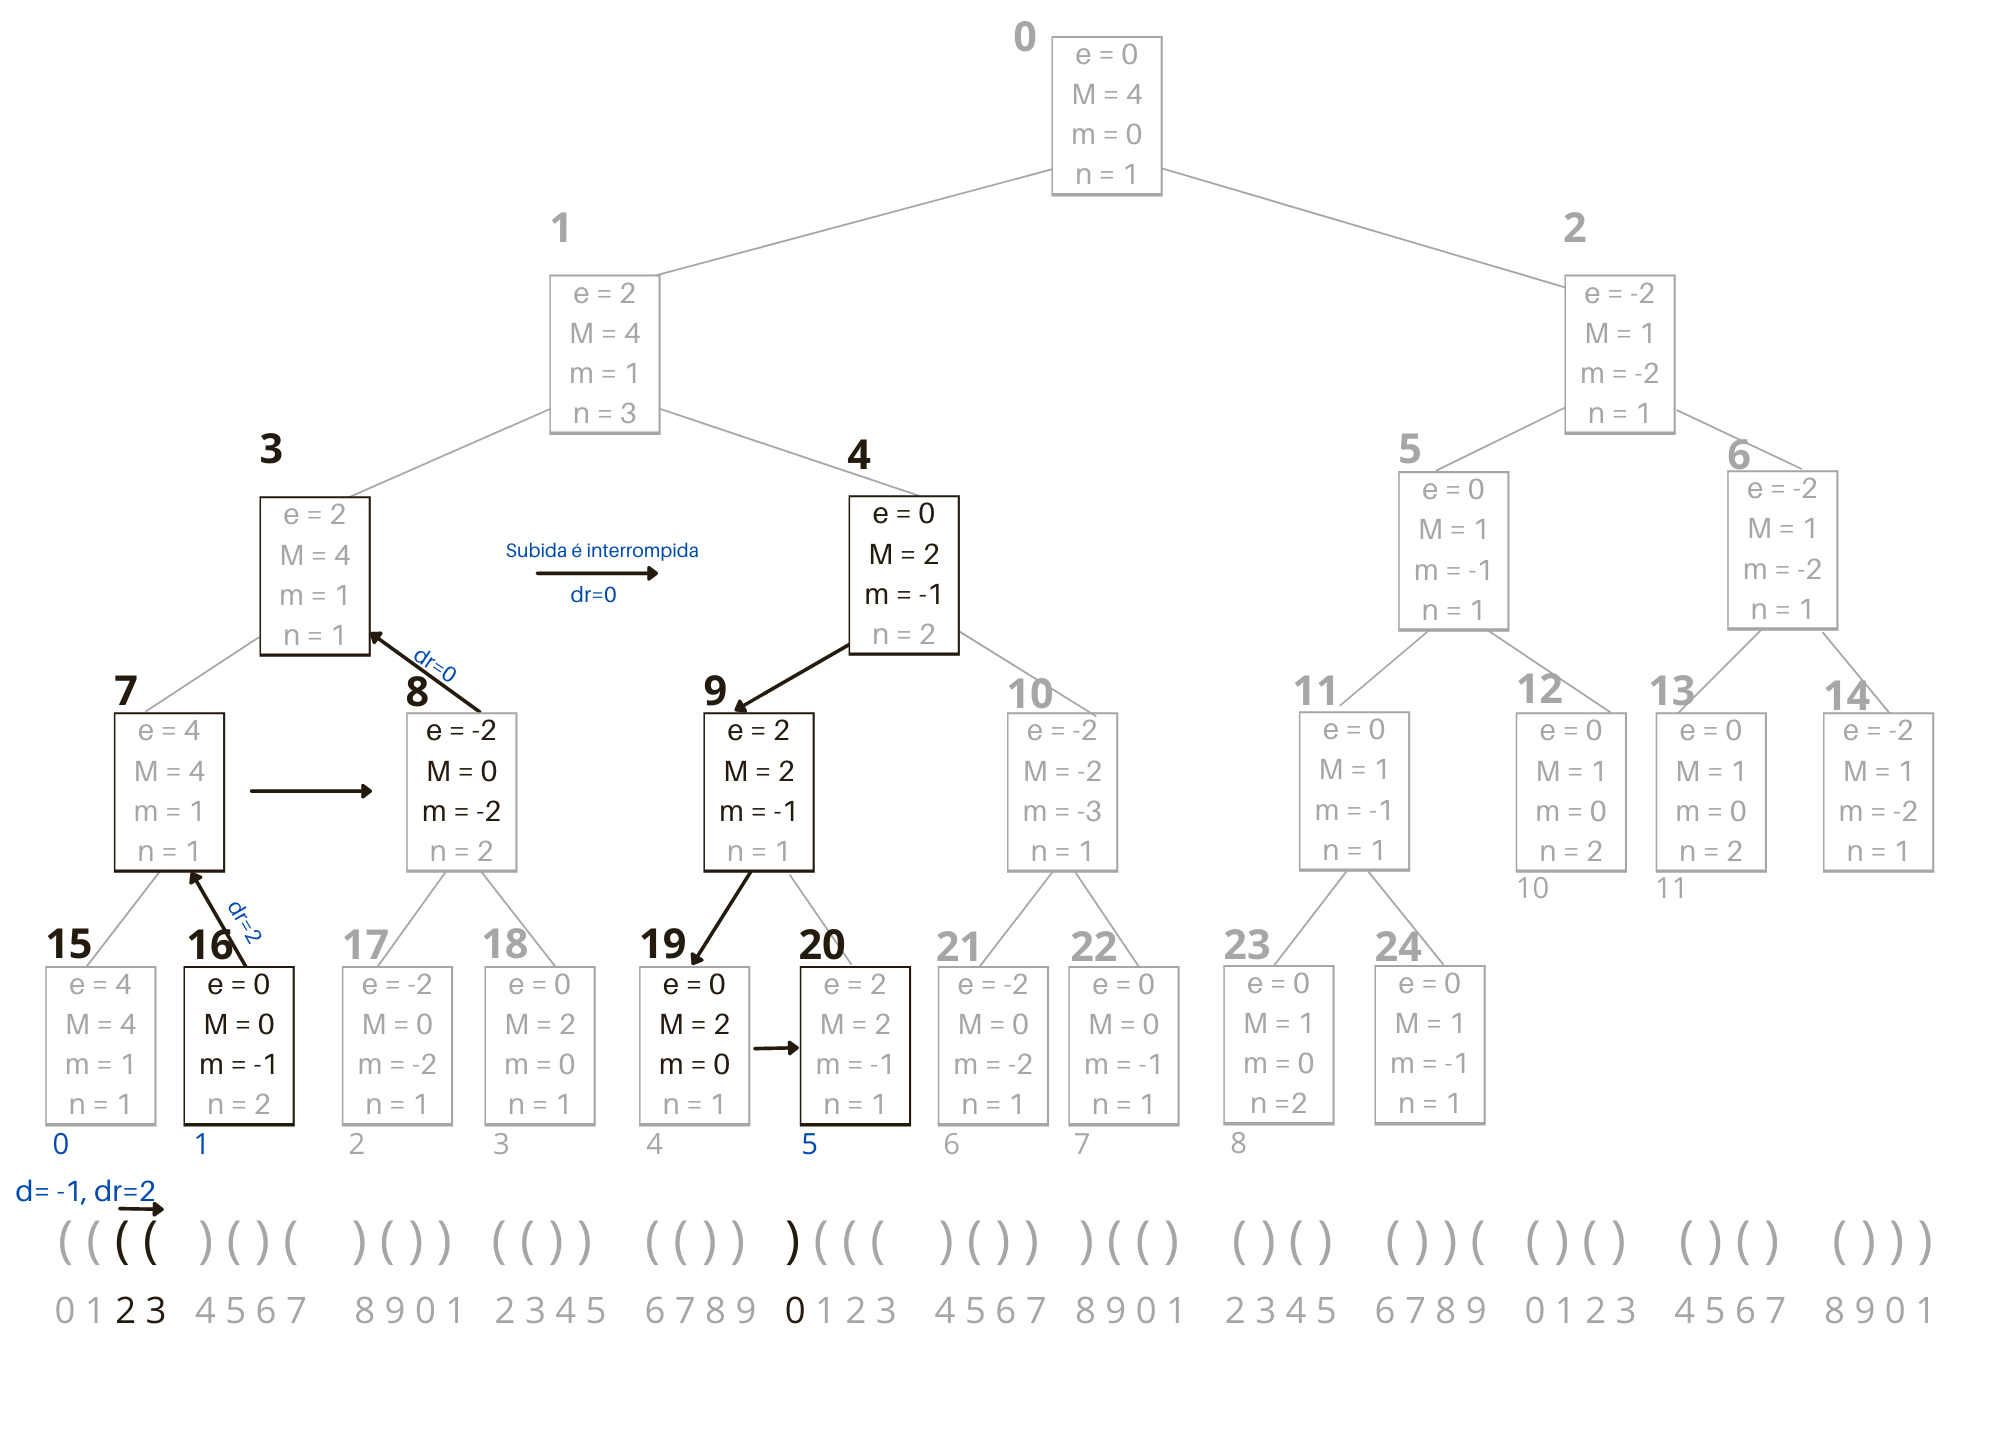
\includegraphics[scale=0.27]{images/rmm-tree-bin-fwdSearch.png}\\
         \caption{Simulação de $fwdSearch(1,-1)=20$ usando a rmM-tree binária}
     \end{figure} 
 \end{frame}



\begin{frame}{Resultados}
    % Please add the following required packages to your document preamble:
% \usepackage[table,xcdraw]{xcolor}
% If you use beamer only pass "xcolor=table" option, i.e. \documentclass[xcolor=table]{beamer}
\begin{table}[]
    \centering
    \caption[Tempo médio de operações]{Tempo (ns) médio de operações sobre o conjunto de dados Complete tree (ctree)}
    \begin{tabular}{lllll}
    \hline
    \multicolumn{1}{l}{\textbf{Operação}} & \multicolumn{1}{l}{\textbf{Binária}} & \multicolumn{1}{l}{\textbf{4-ária}} & \multicolumn{1}{c}{\textbf{8-ária}} & \multicolumn{1}{l}{\textbf{16-ária}} \\ \hline
    fwdSearch                               & 261,58                                & 325,06                               & 317,77                               & 318,34                                \\
    \rowcolor[HTML]{EFEFEF} 
    bwdSearch                               & 1679,19                                & 3200,95                              & 4032,87                              & 6027,23                               \\
    findClose                               & 334.38                                & 399,62                               & 396,91                               & 394,57                                \\
    \rowcolor[HTML]{EFEFEF} 
    findOpen                                & 381,89                                & 443,55                               & 443,54                               & 439,59                                \\
    enclose                                 & 325,01                                & 375,02                               & 377,77                               & 373,34                                \\
    \rowcolor[HTML]{EFEFEF} 
    isAncestor                              & 237,69                                & 264,61                               & 267,17                               & 266,70                                \\
    parent                                  & 327,19                                & 377,9                                & 378,63                               & 372,16                 \\ 
    \rowcolor[HTML]{EFEFEF} 
    subTreeSize                             & 352,38                                & 417,97                               & 418,75                               & 417,01                                \\
    %\rowcolor[HTML]{EFEFEF} 
    nextSibling                             & 264,41                                & 288,8,78                             & 287,45                               & 289,87                                \\ \hline            
    \end{tabular}
    \end{table}
\end{frame}


\begin{frame}{Resultados}
    % Please add the following required packages to your document preamble:
% \usepackage[table,xcdraw]{xcolor}
% If you use beamer only pass "xcolor=table" option, i.e. \documentclass[xcolor=table]{beamer}
\begin{table}[]
    \centering
    \caption[Tempo médio de operações]{Tempo (ns) médio de operações sobre o conjunto de dados Complete tree (ctree)}
    \begin{tabular}{lllll}
    \hline
    \multicolumn{1}{l}{\textbf{Operação}} & \multicolumn{1}{l}{\textbf{Binária}} & \multicolumn{1}{l}{\textbf{4-ária}} & \multicolumn{1}{c}{\textbf{8-ária}} & \multicolumn{1}{l}{\textbf{16-ária}} \\ \hline
    prevSibling                             & 240,24                                & 266,53                               & 268,30                               & 265,65                                \\
    \rowcolor[HTML]{EFEFEF} 
    lastChild                               & 395,22                                & 436,02                               & 437,15                               & 436,34                                \\
    levelNext                               & 366,81                                & 452,55                               & 450,61                               & 442,64                                \\
    \rowcolor[HTML]{EFEFEF} 
    levelAncestor                           & 882,93                                & 1656,51                              & 2089,76                              & 3113,49                               \\
    postRank                                & 177,92                                & 176,93                               & 174,66                               & 184,18                                \\
    \rowcolor[HTML]{EFEFEF} 
    postSelect                              & 844,9                                 & 911,84                               & 919,35                             & 372,16                 \\ \hline              
    \end{tabular}
    \end{table}
\end{frame}

\begin{frame}{Resultados}  
    \begin{figure}[h!]
        \centering
        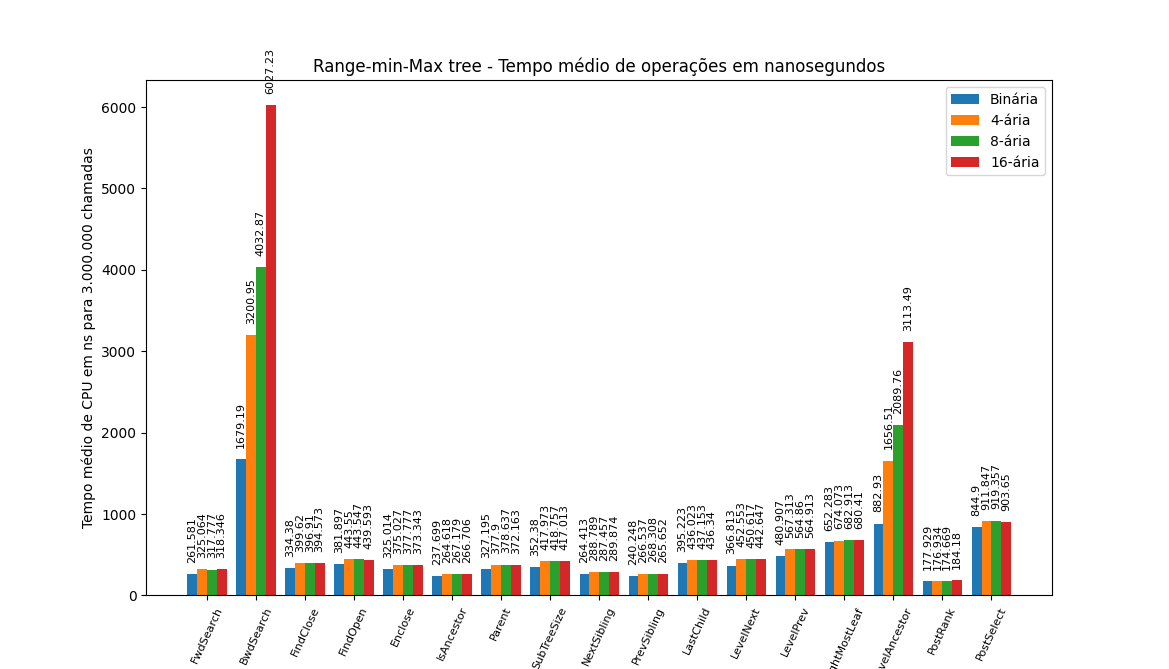
\includegraphics[scale=0.35]{images/ctree_i3000000.png}\\
        \caption{Tempo médio para $3.000.000$ requisições sobre o conjunto de dados Complete tree (ctree)}
    \end{figure} 
\end{frame}

\section{Trabalhos futuros}

\begin{frame}{Trabalhos futuros}
    \begin{itemize}
        \item Redução do tempo das operações da rmM-tree;
        \item Implementar demais operações para a rmM-tree k-ária;
        \item Monitorar uso da cache;
        \item Impacto da proposta em diferentes ambientes.
    \end{itemize}
\end{frame}



\begin{frame}[allowframebreaks]{Referências}
    \bibliographystyle{plainnat}
    \bibliography{bib/references}
\end{frame}


\begin{frame}{}
    \centering
  \textbf{Obrigada pela atenção!}
  
  \vspace{0.4cm}
  
  \rule[0.4cm]{6cm}{0.6pt}
  
  \textbf{Perguntas}
\end{frame}
\end{document}